\documentclass[11pt,a4paper]{article}
\usepackage[margin=2.5cm]{geometry}
\usepackage{booktabs}
\usepackage{graphicx}
\usepackage{subcaption}
\usepackage{hyperref}
\usepackage{amsmath}
\usepackage{float}
\usepackage{xcolor}
\usepackage{array}
\usepackage{multirow}
\usepackage{longtable}
\usepackage{caption}
\hypersetup{colorlinks=true,linkcolor=blue,urlcolor=blue,citecolor=blue}
\title{\textbf{Adaptive Performance Regression Detection\\
on Firefox-Android Telemetry Data}\\[0.4em]
\large Algorithm~3 Controller: ARIMA vs.\ LAST vs.\ SMA vs.\ EWMA\\
\normalsize Extended Evaluation with Train/Test Split, Precision/Recall/F1,\\
False-Alarm Rate, Detection Delay Distribution, and Compute Cost}
\author{Experimental Evaluation Report}
\date{March 2026}
\begin{document}
\maketitle
\tableofcontents
\newpage

\section{Introduction}

This report presents the extended experimental evaluation of an adaptive
performance-regression detection algorithm applied to the Mozilla
Firefox-Android Treeherder telemetry dataset.  The goal is to decide, at
each new measurement point~$t$, whether to \emph{record} a sample
(``enable'' the sensor) based on an exponential anomaly score derived from
the one-step-ahead forecast residual.

Five forecasting strategies are compared inside \textbf{Algorithm~3}:
\begin{itemize}
  \item \textbf{ARIMA}$(p,d,q)=(1,1,1)$ --- parameters estimated on the
        training split only; a fixed-parameter Kalman filter is rolled
        forward on the test set (no data leakage).
  \item \textbf{LAST} (na\"{i}ve baseline) --- $\hat{y}_t = y_{t-1}$.
  \item \textbf{SMA}$(w)$ --- simple moving average over the last $w$ points.
  \item \textbf{EWMA}$(\alpha)$ --- exponentially weighted moving average:
        $\hat{y}_t = \alpha\,y_{t-1} + (1{-}\alpha)\,\hat{y}_{t-1}$.
  \item \textbf{Transformer} --- sequence-model forecaster evaluated under the
        same alert-matching and storage-reduction protocol.
\end{itemize}

This evaluation adds over the previous study:
\begin{itemize}
  \item Strict \textbf{chronological train/test split} with leakage controls.
  \item \textbf{Precision}, \textbf{Recall}, \textbf{F1} on the test set.
  \item \textbf{False-alarm rate} (FP intervals per test time step).
  \item Full \textbf{detection-delay distribution} statistics.
  \item \textbf{Compute and peak memory} measurements.
\end{itemize}


\section{Dataset and Parameters}

\subsection{Dataset Statistics}


\begin{table}[H]
\centering
\caption{Dataset statistics.}
\label{tab:dataset}
\begin{tabular}{lr}
\toprule
Metric & Value \\
\midrule
Total alert records              & 17,989 \\
Regression alert records         & 7,612 \\
Unique regression signatures     & 3,764 \\
Timeseries CSV files available   & 342 \\
Signatures matched to timeseries & 214 \\
Vectors converted and used       & 214 \\
\bottomrule
\end{tabular}
\end{table}


\subsection{Algorithm Parameters}


\begin{table}[H]
\centering
\caption{Shared Algorithm~3 parameters.}
\label{tab:params}
\begin{tabular}{lll}
\toprule
Parameter & Symbol & Value \\
\midrule
Exponential weight      & $\beta$                            & 0.3 \\
Detection threshold     & $\theta_{\mathrm{anomaly}}$   & 0.3 \\
Dynamic threshold scale & $k_\sigma$                         & 3.0 \\
Dynamic threshold window & $w_{\mathrm{thr}}$            & 30 \\
ARIMA order $(p,d,q)$   & ---                                 & (1, 1, 1) \\
ARIMA min.\ history    & $h_{\min}$                       & 20 \\
ARIMA rolling window    & $w_{\mathrm{ARIMA}}$           & 60 \\
SMA window              & $w_{\mathrm{SMA}}$             & 20 \\
EWMA smoothing          & $\alpha$                           & 0.3 \\
Alert tolerance         & $\tau$                             & $\pm5$\,pushes \\
Train fraction          & ---                                 & 70\% \\
Test fraction           & ---                                 & 30\% \\
\bottomrule
\end{tabular}
\end{table}


\section{Methodology}

\subsection{Algorithm~3 Controller}

At each test-set time step~$t$:
\begin{enumerate}
  \item Compute forecast $\hat{y}_t$ using the chosen method.
  \item Compute residual $\delta_t = |y_t - \hat{y}_t|$.
  \item Compute dynamic threshold
        $\Theta_t = \max\!\left(\Theta_{\min},\, k_\sigma\,\sigma(\delta_{t-w:t})\right)$.
  \item Update anomaly score
        $s_t = \beta\,\mathbf{1}[\delta_t > \Theta_t] + (1{-}\beta)\,s_{t-1}$.
  \item Output \emph{decision}$_t = \mathbf{1}[s_t \geq \theta_{\mathrm{anomaly}}]$.
\end{enumerate}

\subsection{EWMA Forecaster}

\[
  \hat{y}_{t+1} = \alpha\,y_t + (1{-}\alpha)\,\hat{y}_t,\qquad
  \alpha \in (0,1).
\]
The running state is initialised on the training split and carried
forward into the test set without reinitialisation.

\subsection{Train/Test Split and Leakage Controls}


Each time series is split chronologically at the 70\% mark:


\begin{itemize}
  \item \textbf{Train set}: ARIMA parameters are estimated here;
        the dynamic-threshold residual history is seeded from train
        residuals; EWMA state is initialised.
  \item \textbf{Test set}: All detection decisions are evaluated here.
        For ARIMA, the Kalman filter uses \emph{fixed} parameters from
        the train fit --- no re-estimation.  Alert timestamps are compared
        to test-set decisions only during post-hoc evaluation (never used
        for parameter tuning).
\end{itemize}

\subsection{Evaluation Metrics}

\paragraph{Precision and Recall (interval/alert level).}
Contiguous \emph{decision}$=1$ runs form \emph{detected intervals}.
An interval is a TP if it covers a ground-truth alert within $\pm\tau$
pushes; otherwise it is a FP.  An alert with no covering interval is FN.
\[
  \mathrm{Precision} = \frac{\mathrm{TP}_{\mathrm{ivs}}}
                            {\mathrm{TP}_{\mathrm{ivs}}+\mathrm{FP}_{\mathrm{ivs}}},
  \quad
  \mathrm{Recall}    = \frac{\mathrm{TP}_{\mathrm{alerts}}}
                            {\mathrm{TP}_{\mathrm{alerts}}+\mathrm{FN}_{\mathrm{alerts}}},
  \quad
  F_1               = \frac{2\,\mathrm{P}\,\mathrm{R}}{\mathrm{P}+\mathrm{R}}.
\]

\paragraph{False-alarm rate.}
FP intervals divided by test-set length (FP intervals per time step).

\paragraph{Detection delay.}
For each TP alert at time $t_a$ covered by an interval starting at $s$,
delay $d = s - t_a$ (negative = pre-detection).

\paragraph{Storage reduction.}
$1 - (\text{fraction of test-set points with decision}=1)$.


\section{Results}

\subsection{Aggregate Overview}


\begin{table}[H]
\centering
\caption{Aggregate metrics on the test set. Higher detection rate and
  lower enabled fraction (higher storage reduction) are both desirable.}
\label{tab:agg}
\begin{tabular}{lrrrrrrrr}
\toprule
Method & Sigs & Alert. & Det. & Det.\,Rate (\%) & Stor.\,Red. & En.\,Frac. & Uniq.\,Chg \\
\midrule
ARIMA(1,1,1) & 214 & 150 & 133 & 88.7 & 89.8\% & 10.2\% & 10.3 \\
LAST (na\"ive) & 214 & 150 & 109 & 72.7 & 89.4\% & 10.6\% & 10.0 \\
SMA($w=20$) & 214 & 150 & 144 & 96.0 & 88.8\% & 11.2\% & 10.2 \\
EWMA($\\alpha=0.3$) & 214 & 150 & 124 & 82.7 & 91.0\% & 9.0\% & 10.7 \\
Transformer & 214 & 150 & 72 & 48.0 & 68.6\% & 31.4\% & 2.7 \\
\bottomrule
\end{tabular}
\end{table}


\subsection{Precision, Recall, and F\textsubscript{1}}

\begin{table}[H]
\centering
\caption{Mean per-signature precision, recall, and $F_1$ on the test set.}
\label{tab:prf}
\begin{tabular}{lrrr}
\toprule
Method & Precision & Recall & $F_1$ \\
\midrule
ARIMA(1,1,1) & 0.106 & 0.606 & 0.174 \\
LAST (na\"ive) & 0.079 & 0.484 & 0.133 \\
SMA($w=20$) & 0.112 & 0.657 & 0.185 \\
EWMA($\\alpha=0.3$) & 0.090 & 0.561 & 0.151 \\
Transformer & 0.208 & 0.334 & 0.229 \\
\bottomrule
\end{tabular}
\end{table}


\subsection{False-Alarm Rate}

\begin{table}[H]
\centering
\caption{Mean false-alarm rate (FP detected intervals per test time step).
  Lower is better.}
\label{tab:far}
\begin{tabular}{lr}
\toprule
Method & FAR (per time step) \\
\midrule
ARIMA(1,1,1) & 0.052780 \\
LAST (na\"ive) & 0.052295 \\
SMA($w=20$) & 0.051913 \\
EWMA($\\alpha=0.3$) & 0.055754 \\
Transformer & 0.013004 \\
\bottomrule
\end{tabular}
\end{table}


\subsection{Detection Delay Distribution}

\begin{table}[H]
\centering
\caption{Detection-delay statistics (pushes). Negative = pre-detection.
  Tolerance window: $\pm5$ pushes.}
\label{tab:delay}
\begin{tabular}{lrrrrrrr}
\toprule
Method & Mean & Median & Std & Min & Max & P10 & P90 \\
\midrule
ARIMA(1,1,1) & -2.8 & -2.8 & 0.1 & -2.9 & -2.7 & -2.9 & -2.7 \\
LAST (na\"ive) & -2.3 & -2.3 & 0.1 & -2.4 & -2.3 & -2.4 & -2.3 \\
SMA($w=20$) & -3.2 & -3.2 & 0.1 & -3.3 & -3.1 & -3.3 & -3.1 \\
EWMA($\\alpha=0.3$) & -2.5 & -2.5 & 0.1 & -2.6 & -2.3 & -2.6 & -2.4 \\
Transformer & -42.1 & -42.0 & 3.3 & -45.5 & -38.7 & -44.8 & -39.3 \\
\bottomrule
\end{tabular}
\end{table}


\subsection{Compute and Memory Cost}

\begin{table}[H]
\centering
\caption{Computational cost. Total runtime over all processed signatures;
  mean per-signature peak heap memory (\texttt{tracemalloc}).}
\label{tab:cost}
\begin{tabular}{lrrr}
\toprule
Method & Total runtime (s) & Throughput (sigs/s) & Mean peak mem.\,(KB) \\
\midrule
ARIMA(1,1,1) & 806.41 & 0.3 & 1422.6 \\
LAST (na\"ive) & 23.24 & 9.2 & 83.8 \\
SMA($w=20$) & 29.27 & 7.3 & 90.3 \\
EWMA($\\alpha=0.3$) & 23.13 & 9.3 & 83.9 \\
Transformer & 11024.40 & 0.0 & 633.0 \\
\bottomrule
\end{tabular}
\end{table}


\subsection{Per-Signature Results (Top~10 by Samples Recorded)}


\begin{table}[H]
\centering
\caption{Per-signature metrics --- ARIMA(1,1,1) (top~10 by samples recorded in test set).}
\label{tab:arima_persig}
\begin{tabular}{lrrclrr}
\toprule
Signature & $T$ & $T_{\mathrm{test}}$ & Detected? & Unique & Samples & Stor.\,Red. \\
\midrule
  4654564 & 574 & 173 & Yes & 14 & 115 & 33.5\% \\
  4654567 & 574 & 173 & Yes & 16 & 111 & 35.8\% \\
  4654568 & 574 & 173 & Yes & 17 & 111 & 35.8\% \\
  4654566 & 574 & 173 & Yes & 17 & 45 & 74.0\% \\
  4653782 & 562 & 169 & No & 22 & 38 & 77.5\% \\
  4654594 & 586 & 176 & No & 17 & 37 & 79.0\% \\
  4654581 & 574 & 173 & Yes & 16 & 36 & 79.2\% \\
  4669835 & 2604 & 782 & No & 33 & 36 & 95.4\% \\
  4653867 & 596 & 179 & No & 18 & 34 & 81.0\% \\
  4654045 & 561 & 169 & Yes & 12 & 29 & 82.8\% \\
\bottomrule
\end{tabular}
\end{table}


\begin{table}[H]
\centering
\caption{Per-signature metrics --- LAST (na\"ive) (top~10 by samples recorded in test set).}
\label{tab:last_persig}
\begin{tabular}{lrrclrr}
\toprule
Signature & $T$ & $T_{\mathrm{test}}$ & Detected? & Unique & Samples & Stor.\,Red. \\
\midrule
  4669835 & 2604 & 782 & No & 33 & 36 & 95.4\% \\
  4654397 & 576 & 173 & Yes & 15 & 32 & 81.5\% \\
  4654119 & 593 & 178 & No & 16 & 31 & 82.6\% \\
  4654399 & 576 & 173 & No & 13 & 31 & 82.1\% \\
  4654063 & 606 & 182 & No & 12 & 30 & 83.5\% \\
  4654594 & 586 & 176 & No & 12 & 30 & 83.0\% \\
  4654651 & 577 & 174 & No & 11 & 30 & 82.8\% \\
  4654664 & 594 & 179 & No & 15 & 30 & 83.2\% \\
  4654076 & 606 & 182 & Yes & 15 & 29 & 84.1\% \\
  4654396 & 576 & 173 & Yes & 15 & 29 & 83.2\% \\
\bottomrule
\end{tabular}
\end{table}


\begin{table}[H]
\centering
\caption{Per-signature metrics --- SMA($w=20$) (top~10 by samples recorded in test set).}
\label{tab:sma_persig}
\begin{tabular}{lrrclrr}
\toprule
Signature & $T$ & $T_{\mathrm{test}}$ & Detected? & Unique & Samples & Stor.\,Red. \\
\midrule
  4669835 & 2604 & 782 & No & 27 & 120 & 84.7\% \\
  4654564 & 574 & 173 & Yes & 19 & 98 & 43.4\% \\
  4654567 & 574 & 173 & Yes & 18 & 77 & 55.5\% \\
  4654568 & 574 & 173 & Yes & 18 & 75 & 56.6\% \\
  4653782 & 562 & 169 & No & 16 & 60 & 64.5\% \\
  4654566 & 574 & 173 & Yes & 15 & 40 & 76.9\% \\
  4654074 & 606 & 182 & Yes & 15 & 37 & 79.7\% \\
  4653867 & 596 & 179 & No & 16 & 36 & 79.9\% \\
  4670242 & 612 & 184 & No & 8 & 34 & 81.5\% \\
  4670243 & 612 & 184 & No & 8 & 34 & 81.5\% \\
\bottomrule
\end{tabular}
\end{table}


\begin{table}[H]
\centering
\caption{Per-signature metrics --- EWMA($\\alpha=0.3$) (top~10 by samples recorded in test set).}
\label{tab:ewma_persig}
\begin{tabular}{lrrclrr}
\toprule
Signature & $T$ & $T_{\mathrm{test}}$ & Detected? & Unique & Samples & Stor.\,Red. \\
\midrule
  4669835 & 2604 & 782 & No & 36 & 66 & 91.6\% \\
  4653867 & 596 & 179 & No & 20 & 31 & 82.7\% \\
  4654340 & 613 & 184 & No & 19 & 29 & 84.2\% \\
  4654119 & 593 & 178 & No & 14 & 27 & 84.8\% \\
  4654564 & 574 & 173 & Yes & 19 & 26 & 85.0\% \\
  4654646 & 577 & 174 & No & 17 & 26 & 85.1\% \\
  4654673 & 583 & 175 & Yes & 15 & 25 & 85.7\% \\
  4653864 & 596 & 179 & Yes & 11 & 24 & 86.6\% \\
  4654050 & 561 & 169 & Yes & 13 & 24 & 85.8\% \\
  4654074 & 606 & 182 & Yes & 11 & 24 & 86.8\% \\
\bottomrule
\end{tabular}
\end{table}


\begin{table}[H]
\centering
\caption{Per-signature metrics --- Transformer (top~10 by samples recorded in test set).}
\label{tab:transformer_persig}
\begin{tabular}{lrrclrr}
\toprule
Signature & $T$ & $T_{\mathrm{test}}$ & Detected? & Unique & Samples & Stor.\,Red. \\
\midrule
  4669835 & 2604 & 782 & No & 3 & 778 & 0.5\% \\
  4653888 & 635 & 191 & No & 1 & 191 & 0.0\% \\
  4653890 & 635 & 191 & Yes & 1 & 191 & 0.0\% \\
  4653896 & 635 & 191 & Yes & 1 & 191 & 0.0\% \\
  4654095 & 619 & 186 & Yes & 1 & 186 & 0.0\% \\
  4654101 & 619 & 186 & Yes & 1 & 186 & 0.0\% \\
  4654313 & 614 & 185 & Yes & 1 & 185 & 0.0\% \\
  4654331 & 613 & 184 & Yes & 1 & 184 & 0.0\% \\
  4654345 & 613 & 184 & No & 1 & 184 & 0.0\% \\
  4654325 & 614 & 185 & Yes & 3 & 183 & 1.1\% \\
\bottomrule
\end{tabular}
\end{table}


\section{Statistical Significance}

All statistical comparisons use per-signature metrics on the test set
($n = 214$ matched signatures).


\subsection{Percentile Bootstrap Confidence Intervals (95\,\%)}

\begin{table}[H]
\centering
\caption{Bootstrap 95\,\% confidence intervals (2\,000 resamples, percentile
  method) for the mean of each metric across all 214 test-set signatures.}
\label{tab:ci}
\begin{tabular}{llrr}
\toprule
Method & Metric & Mean & 95\,\% CI \\
\midrule
  ARIMA(1,1,1) & Precision & 0.1056 & [0.0926,~0.1192] \\
  ARIMA(1,1,1) & Recall & 0.6059 & [0.5428,~0.6682] \\
  ARIMA(1,1,1) & $F_1$ & 0.1736 & [0.1538,~0.1947] \\
  ARIMA(1,1,1) & FAR & 0.0528 & [0.0502,~0.0554] \\
  LAST (na\"ive) & Precision & 0.0793 & [0.0673,~0.0916] \\
  LAST (na\"ive) & Recall & 0.4844 & [0.4229,~0.5498] \\
  LAST (na\"ive) & $F_1$ & 0.1330 & [0.1139,~0.1529] \\
  LAST (na\"ive) & FAR & 0.0523 & [0.0503,~0.0545] \\
  SMA($w=20$) & Precision & 0.1116 & [0.0995,~0.1252] \\
  SMA($w=20$) & Recall & 0.6573 & [0.5958,~0.7189] \\
  SMA($w=20$) & $F_1$ & 0.1855 & [0.1663,~0.2061] \\
  SMA($w=20$) & FAR & 0.0519 & [0.0494,~0.0543] \\
  EWMA($\\alpha=0.3$) & Precision & 0.0902 & [0.0777,~0.1033] \\
  EWMA($\\alpha=0.3$) & Recall & 0.5615 & [0.4977,~0.6246] \\
  EWMA($\\alpha=0.3$) & $F_1$ & 0.1506 & [0.1313,~0.1712] \\
  EWMA($\\alpha=0.3$) & FAR & 0.0558 & [0.0533,~0.0581] \\
  Transformer & Precision & --- & --- \\
  Transformer & Recall & --- & --- \\
  Transformer & $F_1$ & --- & --- \\
  Transformer & FAR & --- & --- \\
\bottomrule
\end{tabular}
\end{table}


\subsection{Pairwise Wilcoxon Signed-Rank Tests}

\begin{table}[H]
\centering
\caption{Paired Wilcoxon signed-rank test $p$-values for all six method
  pairs on each metric. Asterisk ($^{*}$) indicates $p < 0.05$.
  Pairs are matched per-signature.}
\label{tab:wilcoxon}
\begin{tabular}{lrrrr}
\toprule
Comparison & Precision & Recall & $F_1$ & FAR \\
\midrule
  ARIMA vs.\ LAST & 0.0000$^{*}$ & 0.0000$^{*}$ & 0.0000$^{*}$ & 0.7651 \\
  ARIMA vs.\ SMA & 0.6524 & 0.0009$^{*}$ & 0.5469 & 0.3803 \\
  ARIMA vs.\ EWMA & 0.0000$^{*}$ & 0.0019$^{*}$ & 0.0000$^{*}$ & 0.0000$^{*}$ \\
  LAST vs.\ SMA & 0.0000$^{*}$ & 0.0000$^{*}$ & 0.0000$^{*}$ & 0.2246 \\
  LAST vs.\ EWMA & 0.0105$^{*}$ & 0.0001$^{*}$ & 0.0061$^{*}$ & 0.0131$^{*}$ \\
  SMA vs.\ EWMA & 0.0000$^{*}$ & 0.0000$^{*}$ & 0.0000$^{*}$ & 0.0000$^{*}$ \\
\bottomrule
\end{tabular}
\end{table}


\section{Ablation Study (Robustness Analysis)}

We vary each hyperparameter individually while keeping the others at their
baseline values.  Post-hoc ablations reuse saved detector outputs; re-run
ablations re-execute the detector with modified settings.


\subsection{Ablation: Anomaly-Score Smoothing Factor~$\beta$}

$\beta$ controls how quickly the exponential anomaly score reacts to
individual anomalous residuals.  Baseline: $\beta = 0.3$.
\textit{Note: scores are reset to~0 at the test-phase boundary for this
ablation.}

\begin{table}[H]
\centering
\caption{$F_1$ score as a function of $\beta$ (all 214 signatures, $\tau=5$, $\theta=0.3$).}
\label{tab:abl_beta_f1}
\begin{tabular}{lrrrr}
\toprule
$\beta$ & ARIMA(1,1,1) & LAST (na\"ive) & SMA($w=20$) & EWMA($\\alpha=0.3$) & Transformer \\
\midrule
  0.100 & 0.182 & 0.017 & 0.410 & 0.040 & --- \\
  0.200 & 0.266 & 0.048 & 0.339 & 0.207 & --- \\
  0.300 & 0.144 & 0.109 & 0.154 & 0.124 & --- \\
  0.500 & 0.144 & 0.108 & 0.156 & 0.119 & --- \\
  0.700 & 0.137 & 0.107 & 0.153 & 0.116 & --- \\
\bottomrule
\end{tabular}
\end{table}

\begin{table}[H]
\centering
\caption{False-alarm rate (FAR) as a function of $\beta$.}
\label{tab:abl_beta_far}
\begin{tabular}{lrrrr}
\toprule
$\\beta$ & ARIMA(1,1,1) & LAST (na\"ive) & SMA($w=20$) & EWMA($\\alpha=0.3$) & Transformer \\\\
\\midrule
  0.100 & 0.00322 & 0.00410 & 0.00486 & 0.00203 & --- \\
  0.200 & 0.01762 & 0.02448 & 0.01799 & 0.01730 & --- \\
  0.300 & 0.05387 & 0.05332 & 0.05318 & 0.05669 & --- \\
  0.500 & 0.05473 & 0.05379 & 0.05398 & 0.05702 & --- \\
  0.700 & 0.05725 & 0.05482 & 0.05651 & 0.05789 & --- \\
\bottomrule
\end{tabular}
\end{table}


\subsection{Ablation: Decision Threshold~$\theta$}

$\theta$ is the anomaly-score cut-off for emitting a detection decision.
Baseline: $\theta = 0.3$.

\begin{table}[H]
\centering
\caption{$F_1$ score as a function of $\theta$ (all 214 signatures, $\tau=5$, $\beta=0.3$).}
\label{tab:abl_thr_f1}
\begin{tabular}{lrrrr}
\toprule
$\theta$ & ARIMA(1,1,1) & LAST (na\"ive) & SMA($w=20$) & EWMA($\\alpha=0.3$) & Transformer \\
\midrule
  0.100 & 0.162 & 0.147 & 0.161 & 0.149 & --- \\
  0.150 & 0.162 & 0.120 & 0.160 & 0.151 & --- \\
  0.200 & 0.160 & 0.111 & 0.159 & 0.148 & --- \\
  0.250 & 0.154 & 0.109 & 0.153 & 0.142 & --- \\
  0.300 & 0.144 & 0.109 & 0.155 & 0.123 & --- \\
  0.400 & 0.272 & 0.046 & 0.342 & 0.201 & --- \\
  0.500 & 0.270 & 0.036 & 0.355 & 0.215 & --- \\
\bottomrule
\end{tabular}
\end{table}

\begin{table}[H]
\centering
\caption{False-alarm rate (FAR) as a function of $\theta$.}
\label{tab:abl_thr_far}
\begin{tabular}{lrrrr}
\toprule
$\\theta$ & ARIMA(1,1,1) & LAST (na\"ive) & SMA($w=20$) & EWMA($\\alpha=0.3$) & Transformer \\\\
\\midrule
  0.100 & 0.04210 & 0.04277 & 0.04117 & 0.04500 & --- \\
  0.150 & 0.04683 & 0.04679 & 0.04598 & 0.04983 & --- \\
  0.200 & 0.04874 & 0.04900 & 0.04809 & 0.05173 & --- \\
  0.250 & 0.05264 & 0.05245 & 0.05174 & 0.05543 & --- \\
  0.300 & 0.05382 & 0.05326 & 0.05308 & 0.05676 & --- \\
  0.400 & 0.01674 & 0.02371 & 0.01820 & 0.01600 & --- \\
  0.500 & 0.01096 & 0.01862 & 0.01178 & 0.00882 & --- \\
\bottomrule
\end{tabular}
\end{table}


\subsection{Ablation: Alert-Matching Tolerance~$\tau$}

$\tau$ is the push-level window used to match a detected interval to a
ground-truth alert.  Baseline: $\tau = 5$ pushes.

\begin{table}[H]
\centering
\caption{$F_1$ score as a function of $\tau$ (all 214 signatures, $\theta=0.3$, $\beta=0.3$).}
\label{tab:abl_tau_f1}
\begin{tabular}{lrrrr}
\toprule
$\tau$ & ARIMA(1,1,1) & LAST (na\"ive) & SMA($w=20$) & EWMA($\\alpha=0.3$) & Transformer \\
\midrule
  1.000 & 0.087 & 0.063 & 0.100 & 0.071 & --- \\
  2.000 & 0.099 & 0.070 & 0.116 & 0.087 & --- \\
  3.000 & 0.110 & 0.084 & 0.123 & 0.096 & --- \\
  5.000 & 0.144 & 0.109 & 0.155 & 0.123 & --- \\
  7.000 & 0.171 & 0.126 & 0.166 & 0.154 & --- \\
  10.000 & 0.187 & 0.164 & 0.179 & 0.165 & --- \\
\bottomrule
\end{tabular}
\end{table}

\begin{table}[H]
\centering
\caption{False-alarm rate (FAR) as a function of $\tau$.}
\label{tab:abl_tau_far}
\begin{tabular}{lrrrr}
\toprule
$\\tau$ & ARIMA(1,1,1) & LAST (na\"ive) & SMA($w=20$) & EWMA($\\alpha=0.3$) & Transformer \\\\
\\midrule
  1.000 & 0.05576 & 0.05470 & 0.05485 & 0.05860 & --- \\
  2.000 & 0.05530 & 0.05449 & 0.05435 & 0.05801 & --- \\
  3.000 & 0.05491 & 0.05407 & 0.05412 & 0.05770 & --- \\
  5.000 & 0.05382 & 0.05326 & 0.05308 & 0.05676 & --- \\
  7.000 & 0.05289 & 0.05268 & 0.05262 & 0.05582 & --- \\
  10.000 & 0.05221 & 0.05141 & 0.05207 & 0.05535 & --- \\
\bottomrule
\end{tabular}
\end{table}


\subsection{Ablation: SMA Window Size~$w$}

The simple-moving-average window $w$ controls the smoothing lag.  Larger
windows reduce noise sensitivity but increase detection lag for sharp shifts.
Baseline: $w = 20$ (\textbf{bold}).
All 214 signatures evaluated.

\begin{table}[H]
\centering
\caption{SMA performance at varying window sizes ($\tau=5$, $\theta=0.3$, $\beta=0.3$).}
\label{tab:abl_sma_win}
\begin{tabular}{lrrrr}
\toprule
$w$ & Precision & Recall & $F_1$ & FAR \\
\midrule
  5 & 0.071 & 0.507 & 0.121 & 0.05749 \\
  10 & 0.081 & 0.572 & 0.140 & 0.05525 \\
  15 & 0.089 & 0.591 & 0.151 & 0.05408 \\
  \textbf{20} & 0.092 & 0.591 & 0.155 & 0.05308 \\
  30 & 0.096 & 0.610 & 0.161 & 0.05254 \\
  50 & 0.089 & 0.594 & 0.151 & 0.05315 \\
\bottomrule
\end{tabular}
\end{table}


\subsection{Ablation: ARIMA Order $(p,d,q)$}

Five ARIMA specifications are compared on a stratified 20-signature
sample (every $\lfloor 214/20 \rfloor$-th signature by descending
length).  Parameters are estimated on the training split only; fixed-parameter
Kalman rolling is used on the test set throughout.
Baseline: $(1,1,1)$ (\textbf{bold}).

\begin{table}[H]
\centering
\caption{ARIMA performance at varying $(p,d,q)$ orders (20-signature sample,
  $\tau=5$, $\theta=0.3$, $\beta=0.3$).}
\label{tab:abl_arima_ord}
\begin{tabular}{lrrrr}
\toprule
$(p,d,q)$ & Precision & Recall & $F_1$ & FAR \\
\midrule
  (1, 0, 0) & 0.057 & 0.450 & 0.100 & 0.06460 \\
  (0, 1, 1) & 0.086 & 0.550 & 0.147 & 0.05544 \\
  (1, 1, 0) & 0.057 & 0.450 & 0.099 & 0.05773 \\
  \textbf{(1, 1, 1)} & 0.094 & 0.550 & 0.158 & 0.05379 \\
  (2, 1, 2) & 0.091 & 0.550 & 0.153 & 0.05449 \\
\bottomrule
\end{tabular}
\end{table}


\section{Sample Visualisations}

The following figures compare all available methods for a selection of signatures.
Upper panel: actual vs.\ predicted values.
Lower panel: anomaly score with decision step-function and threshold.
The green dotted vertical line marks the train/test split.

\subsubsection*{Signature 4669835}
\begin{figure}[H]
\centering
  \begin{subfigure}[b]{0.19\textwidth}
    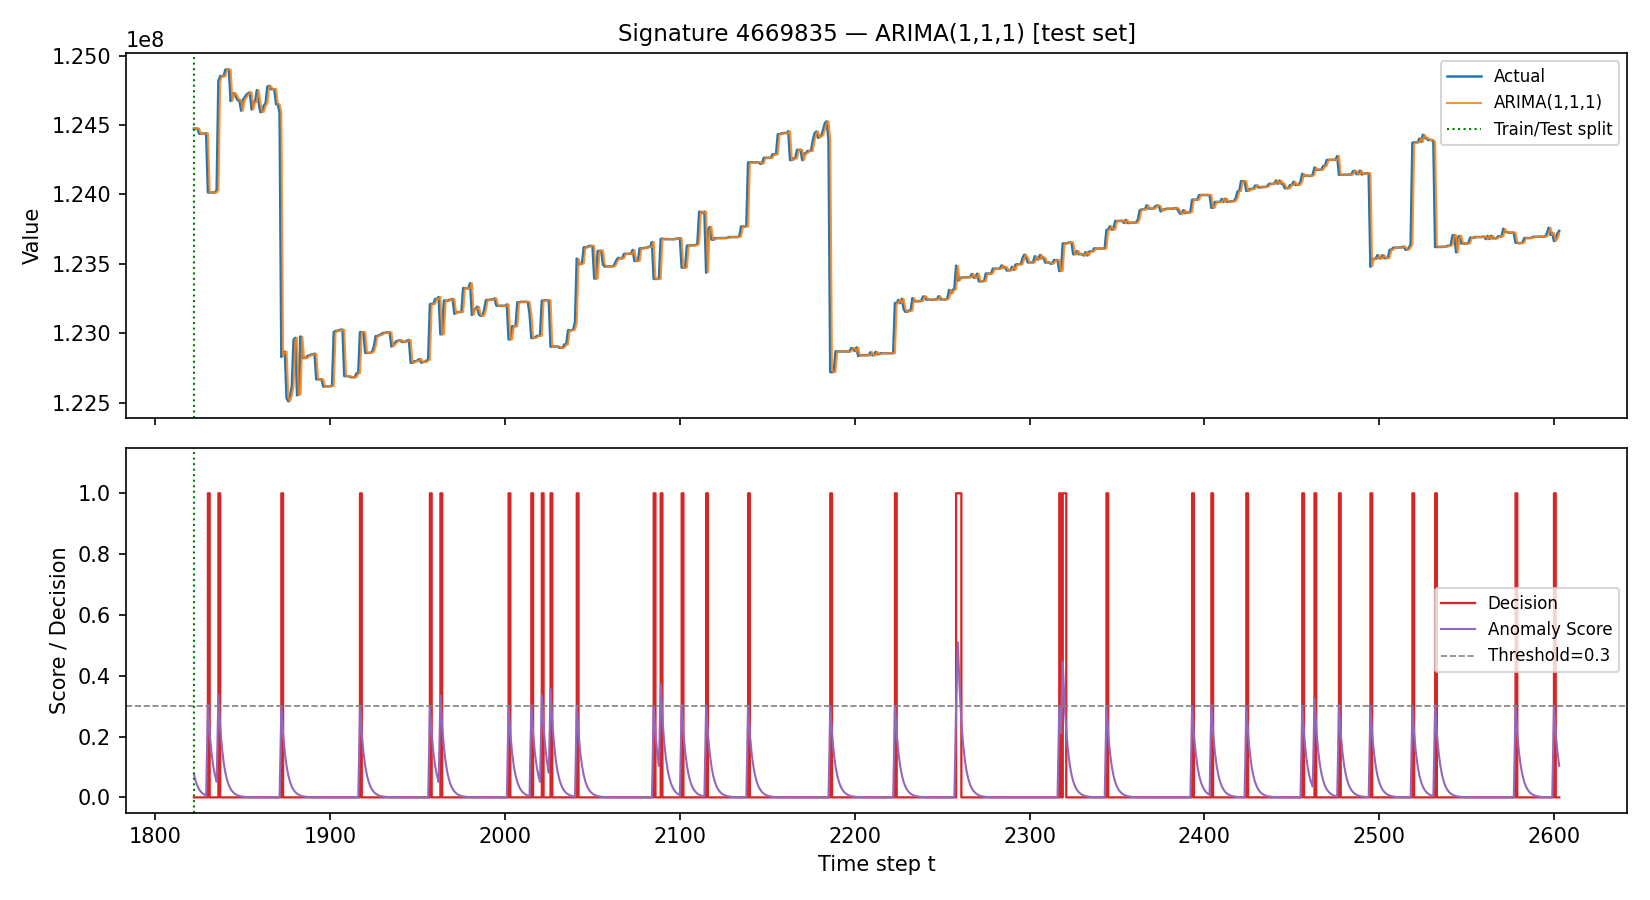
\includegraphics[width=\textwidth]{plots/4669835_arima.png}
    \caption{ARIMA(1,1,1)}
  \end{subfigure}
  \hfill
  \begin{subfigure}[b]{0.19\textwidth}
    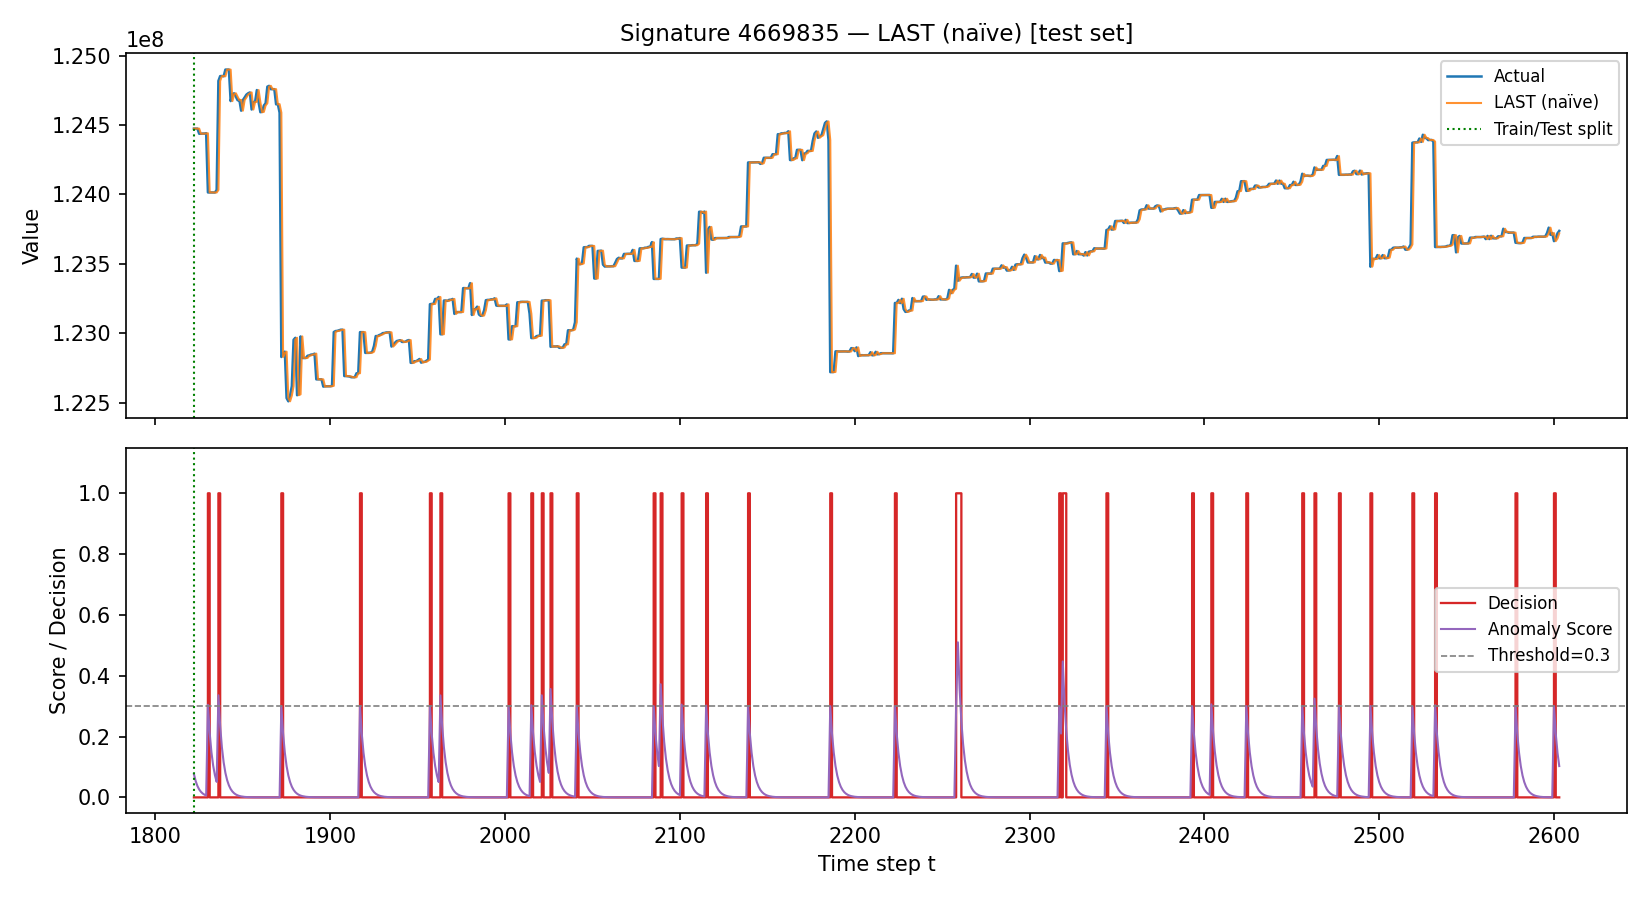
\includegraphics[width=\textwidth]{plots/4669835_last.png}
    \caption{LAST (na\"ive)}
  \end{subfigure}
  \hfill
  \begin{subfigure}[b]{0.19\textwidth}
    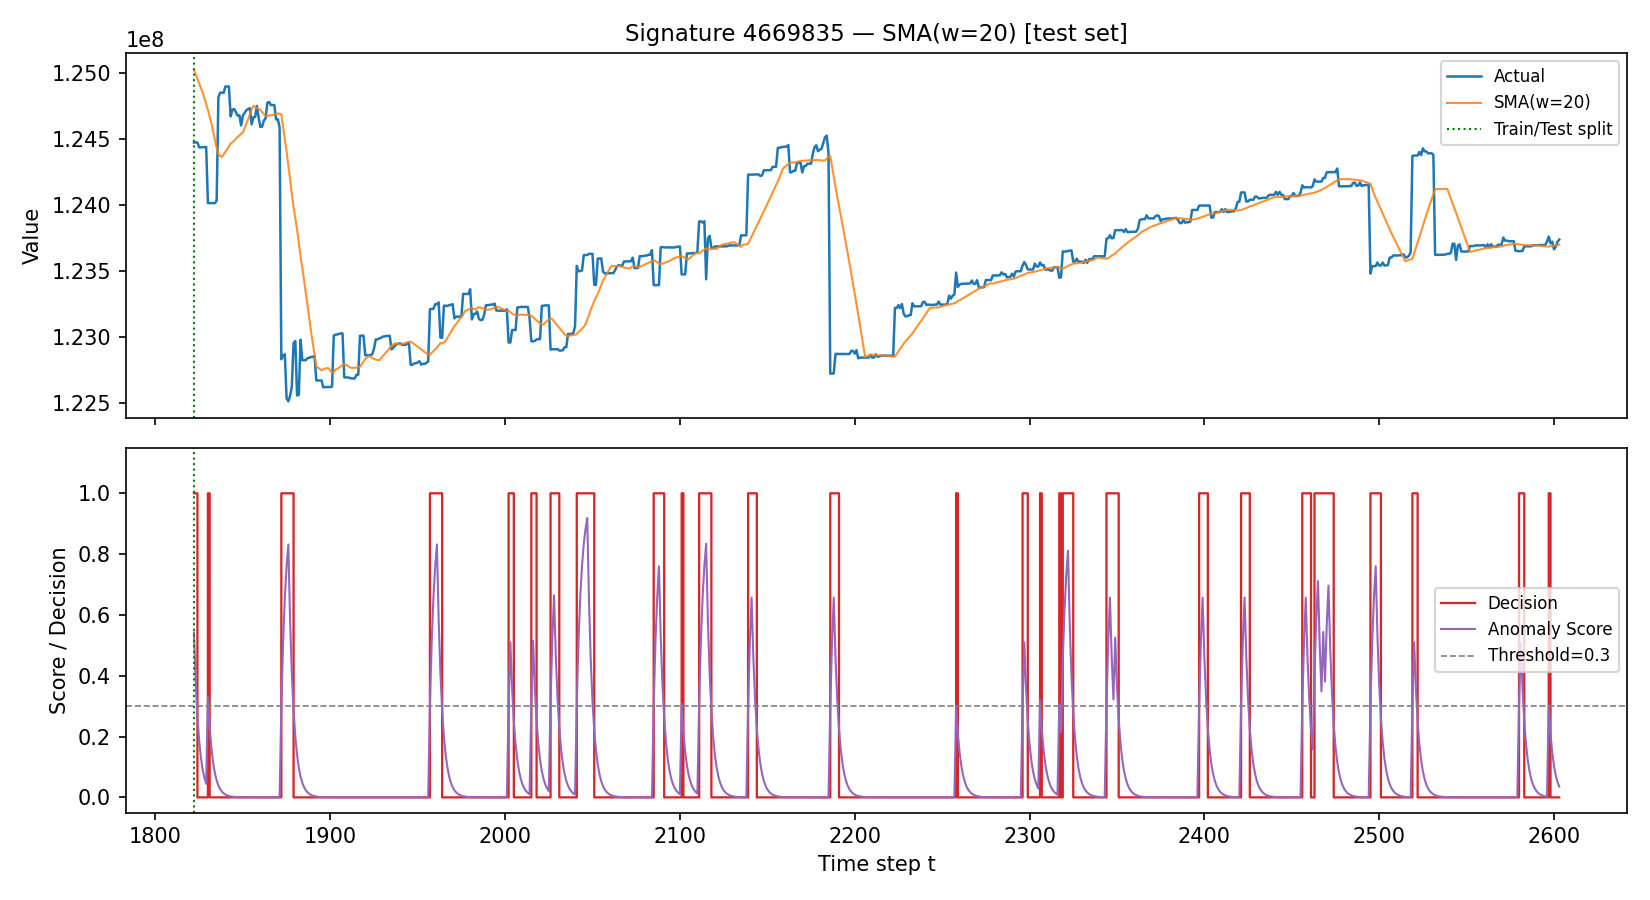
\includegraphics[width=\textwidth]{plots/4669835_sma.png}
    \caption{SMA($w=20$)}
  \end{subfigure}
  \hfill
  \begin{subfigure}[b]{0.19\textwidth}
    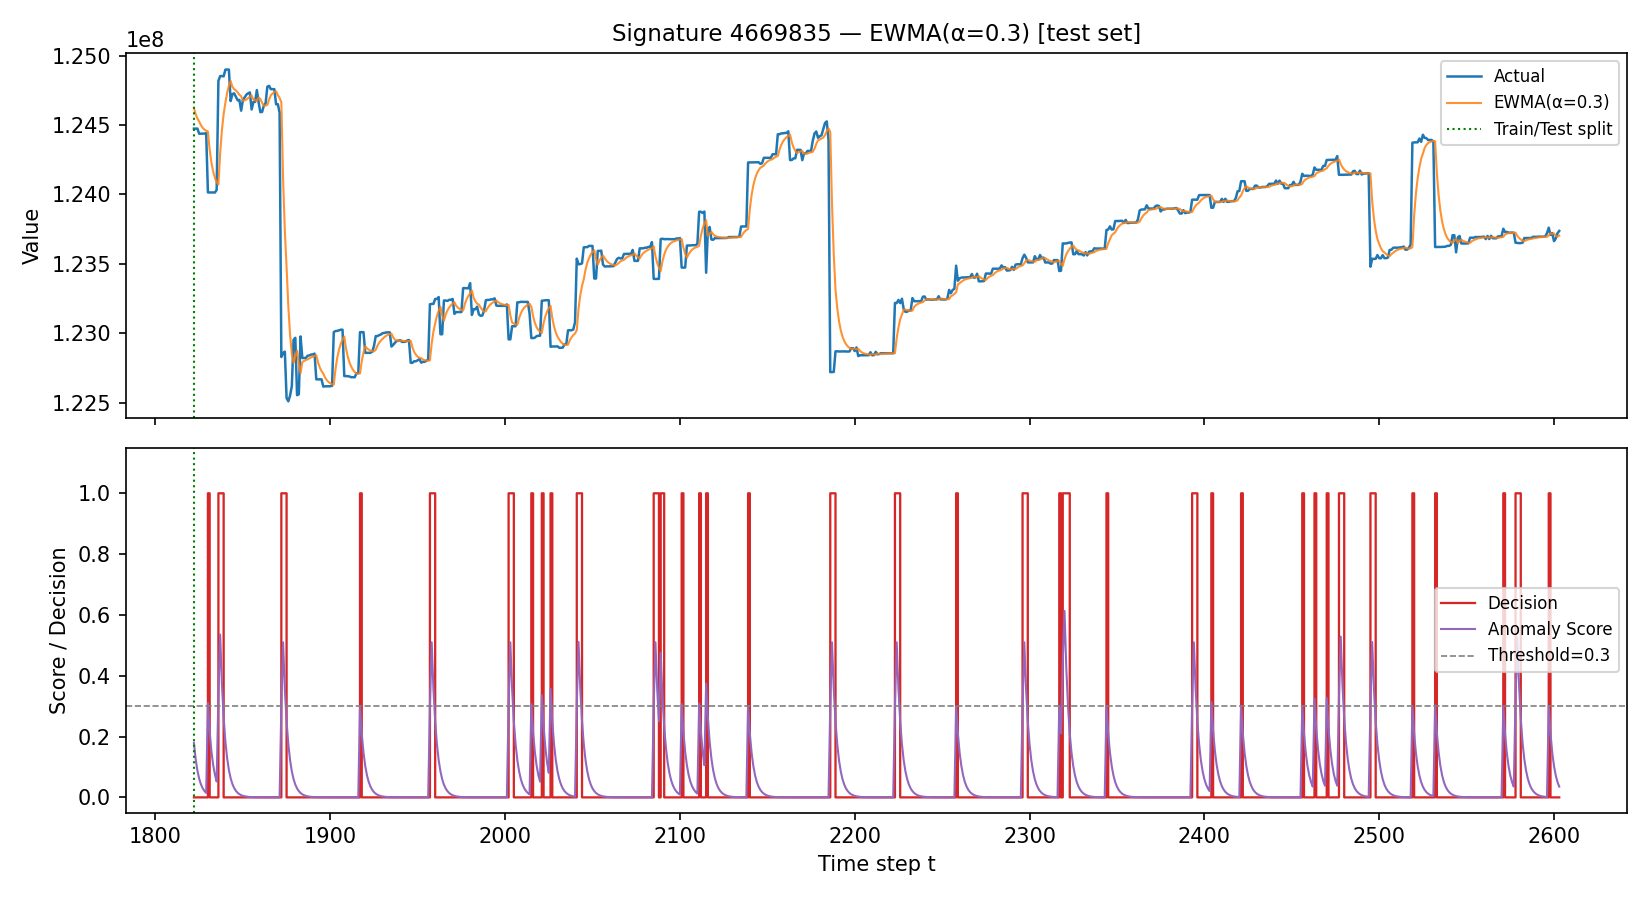
\includegraphics[width=\textwidth]{plots/4669835_ewma.png}
    \caption{EWMA($\\alpha=0.3$)}
  \end{subfigure}
  \hfill
  \begin{subfigure}[b]{0.19\textwidth}
    
\includegraphics[width=\textwidth]{plots/4669835_transformer.png}
    \caption{TRANSFORMER}
  \end{subfigure}
  \caption{Multi-method comparison, signature 4669835.}
  \label{fig:sig0}
\end{figure}

\subsubsection*{Signature 4653879}
\begin{figure}[H]
\centering
  \begin{subfigure}[b]{0.19\textwidth}
    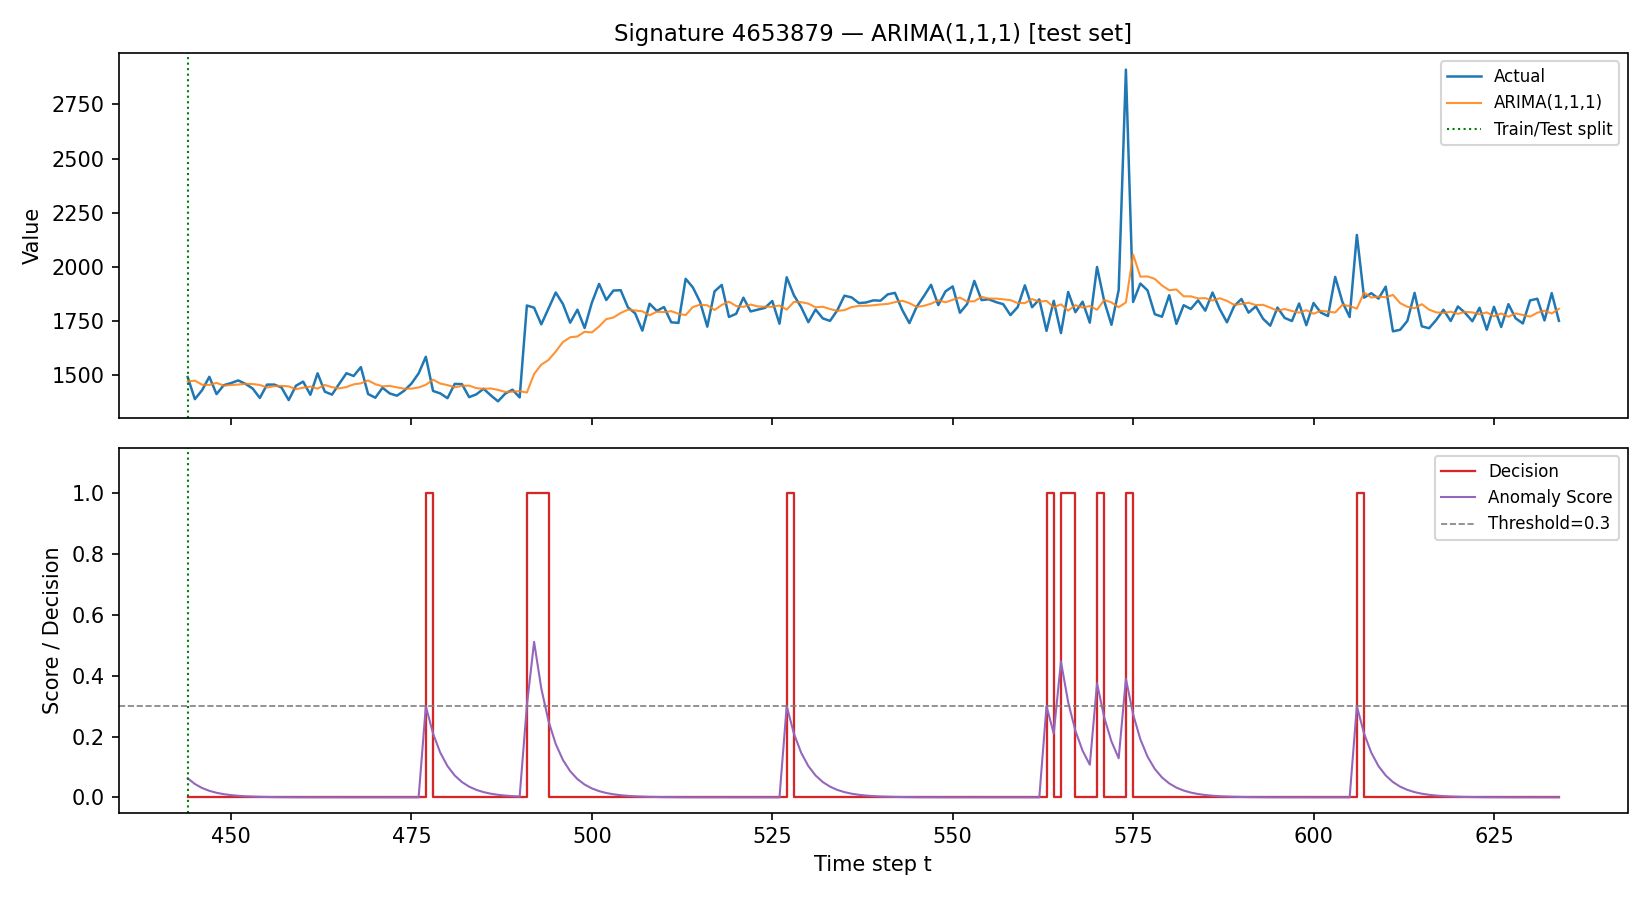
\includegraphics[width=\textwidth]{plots/4653879_arima.png}
    \caption{ARIMA(1,1,1)}
  \end{subfigure}
  \hfill
  \begin{subfigure}[b]{0.19\textwidth}
    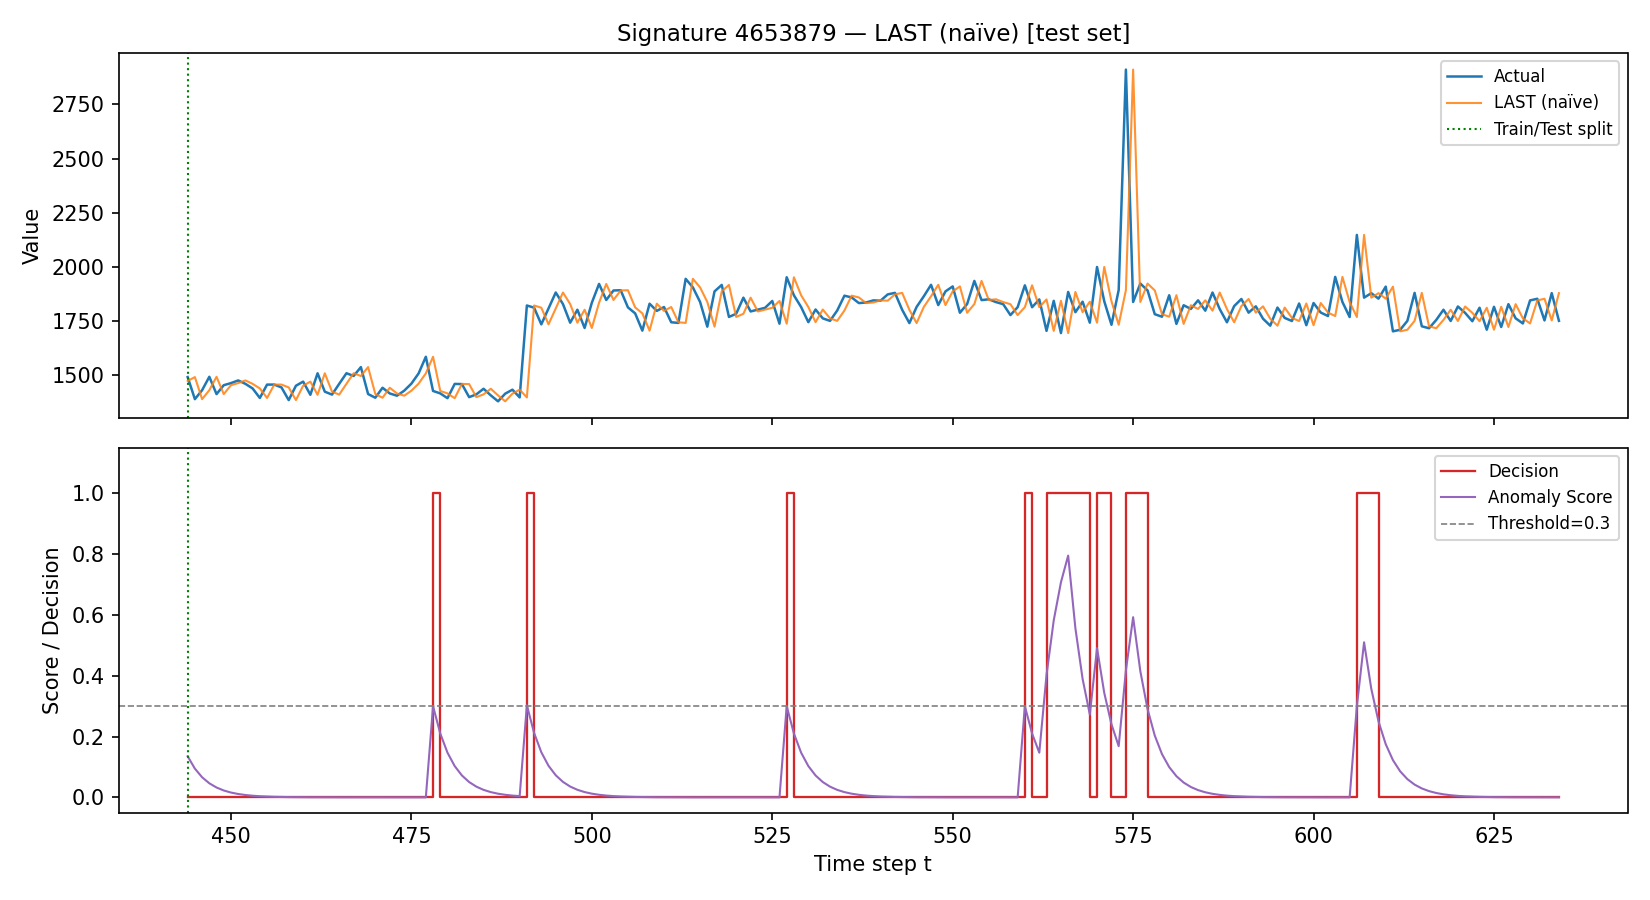
\includegraphics[width=\textwidth]{plots/4653879_last.png}
    \caption{LAST (na\"ive)}
  \end{subfigure}
  \hfill
  \begin{subfigure}[b]{0.19\textwidth}
    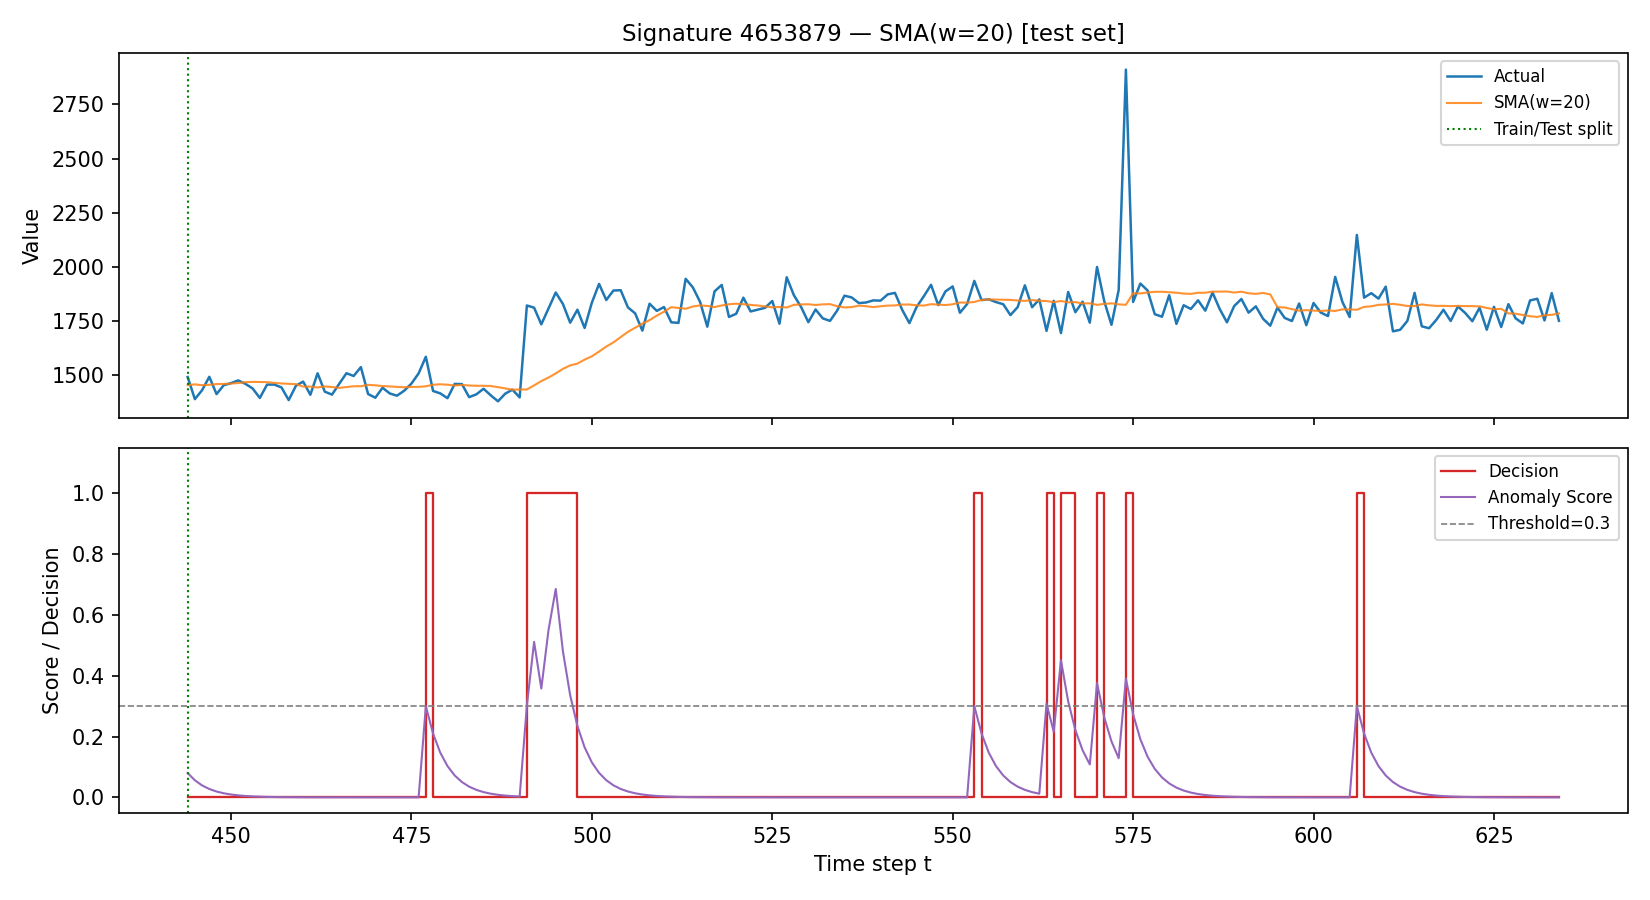
\includegraphics[width=\textwidth]{plots/4653879_sma.png}
    \caption{SMA($w=20$)}
  \end{subfigure}
  \hfill
  \begin{subfigure}[b]{0.19\textwidth}
    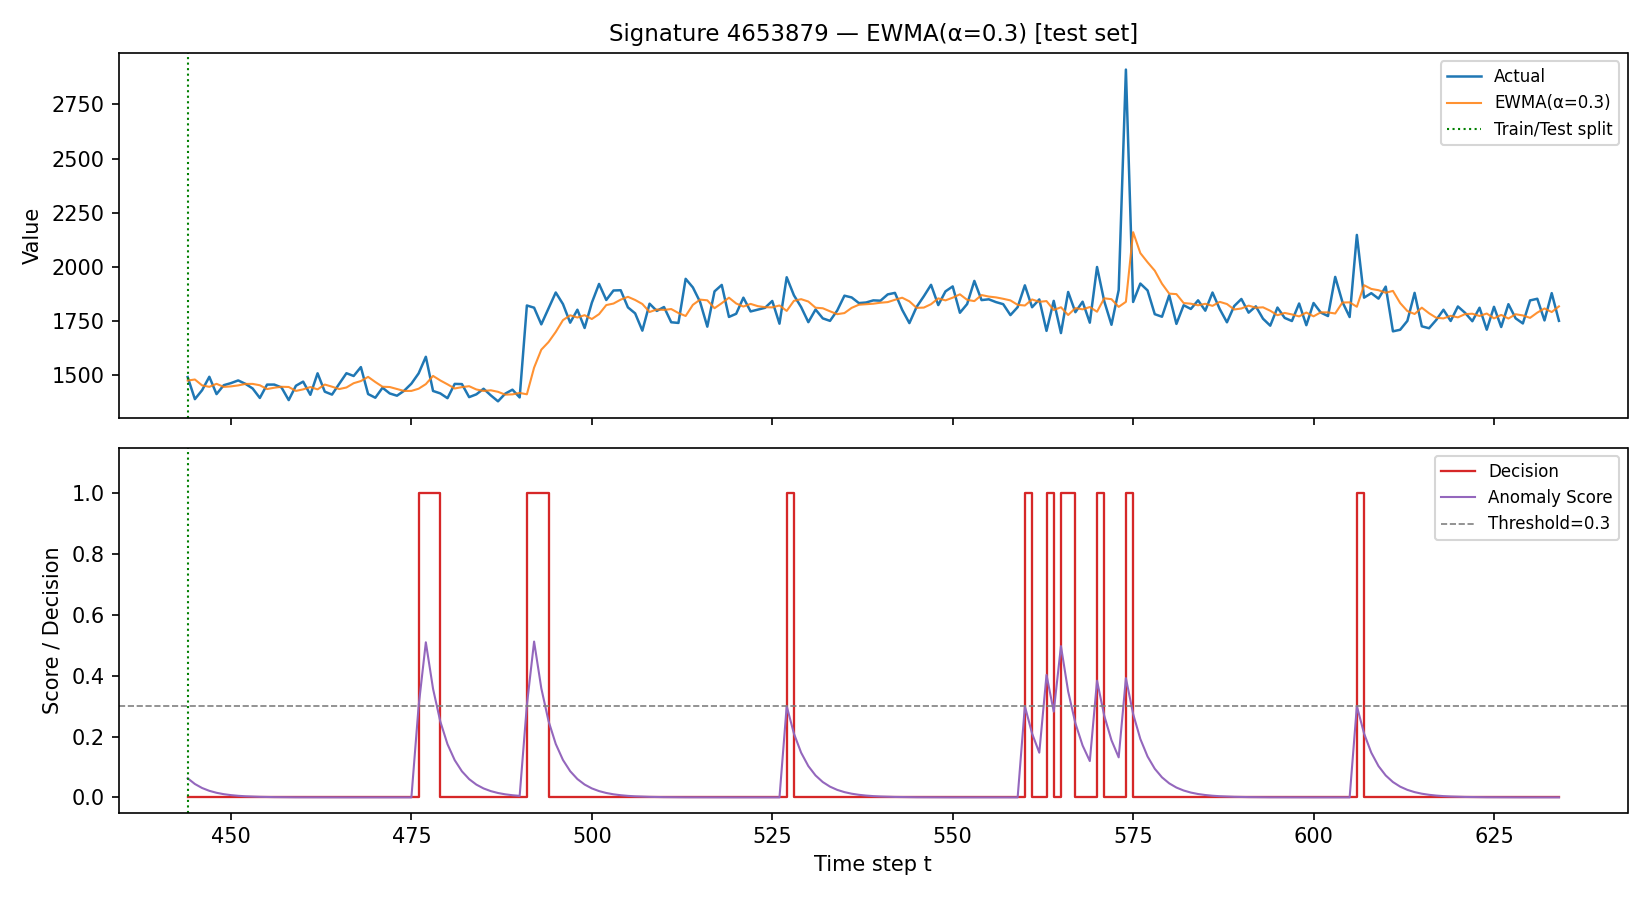
\includegraphics[width=\textwidth]{plots/4653879_ewma.png}
    \caption{EWMA($\\alpha=0.3$)}
  \end{subfigure}
  \hfill
  \begin{subfigure}[b]{0.19\textwidth}
    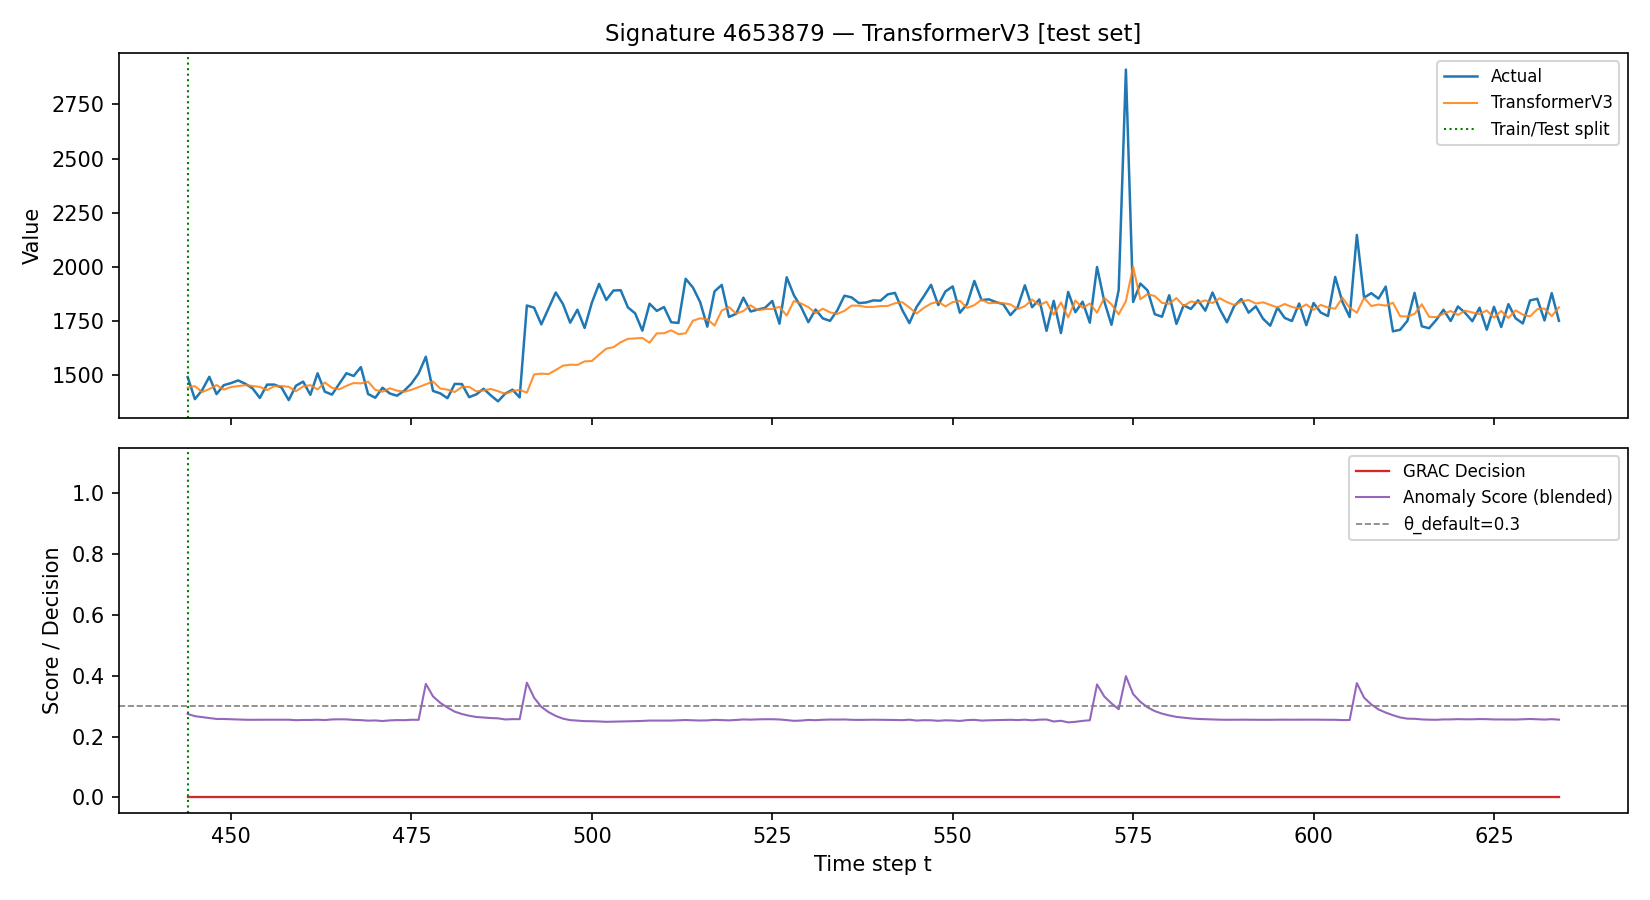
\includegraphics[width=\textwidth]{plots/4653879_transformer.png}
    \caption{TRANSFORMER}
  \end{subfigure}
  \caption{Multi-method comparison, signature 4653879.}
  \label{fig:sig1}
\end{figure}

\subsubsection*{Signature 4653880}
\begin{figure}[H]
\centering
  \begin{subfigure}[b]{0.19\textwidth}
    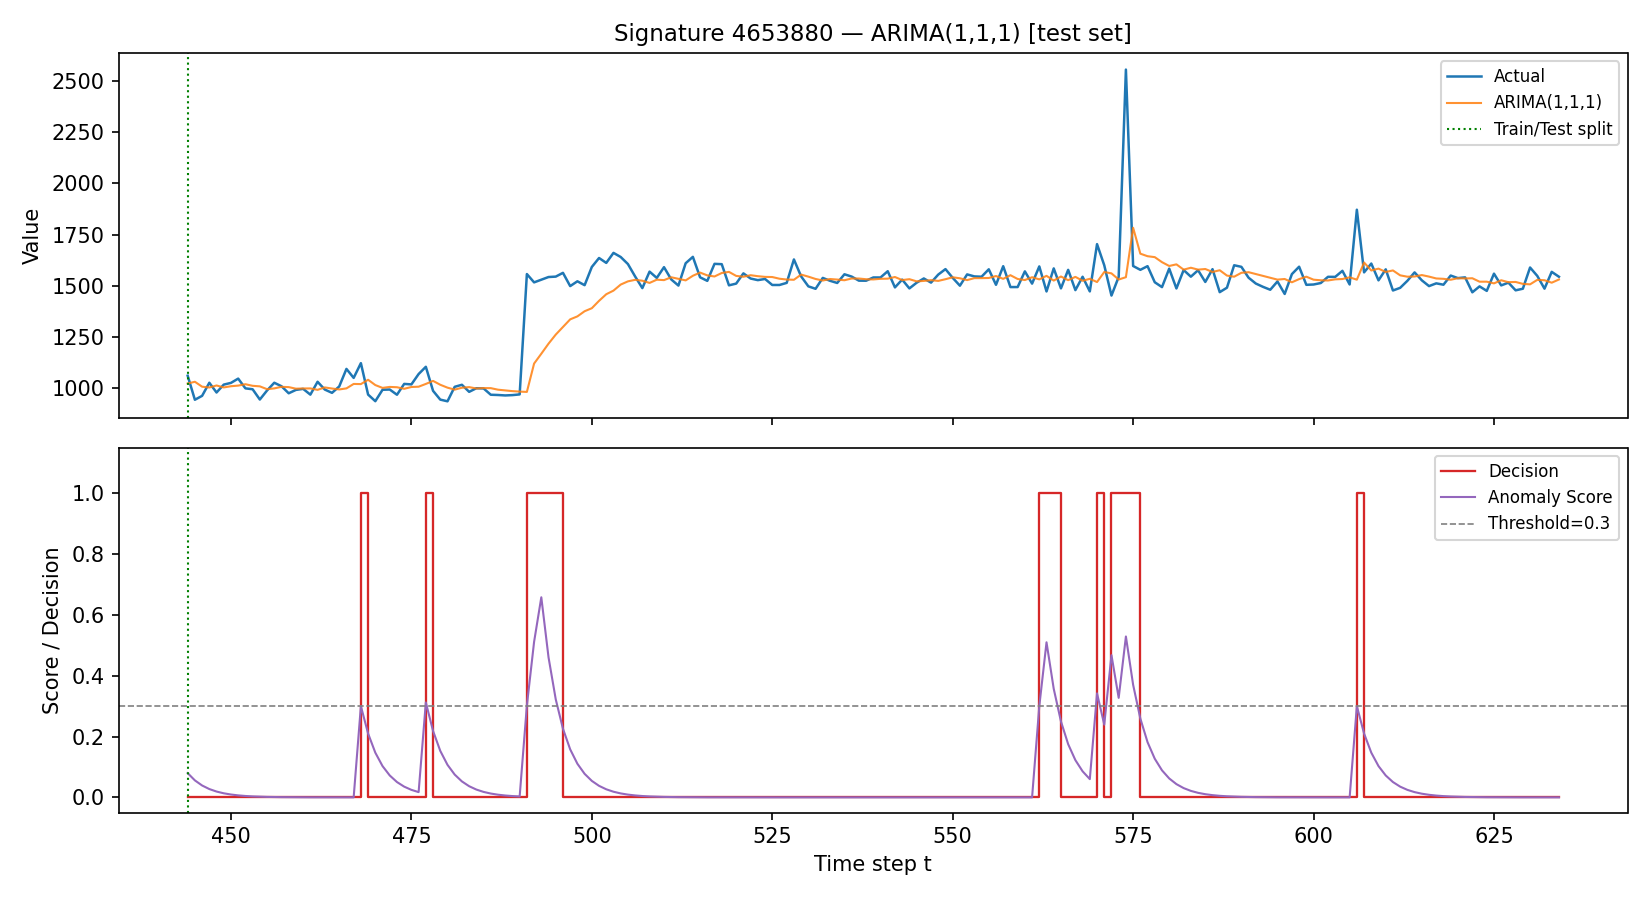
\includegraphics[width=\textwidth]{plots/4653880_arima.png}
    \caption{ARIMA(1,1,1)}
  \end{subfigure}
  \hfill
  \begin{subfigure}[b]{0.19\textwidth}
    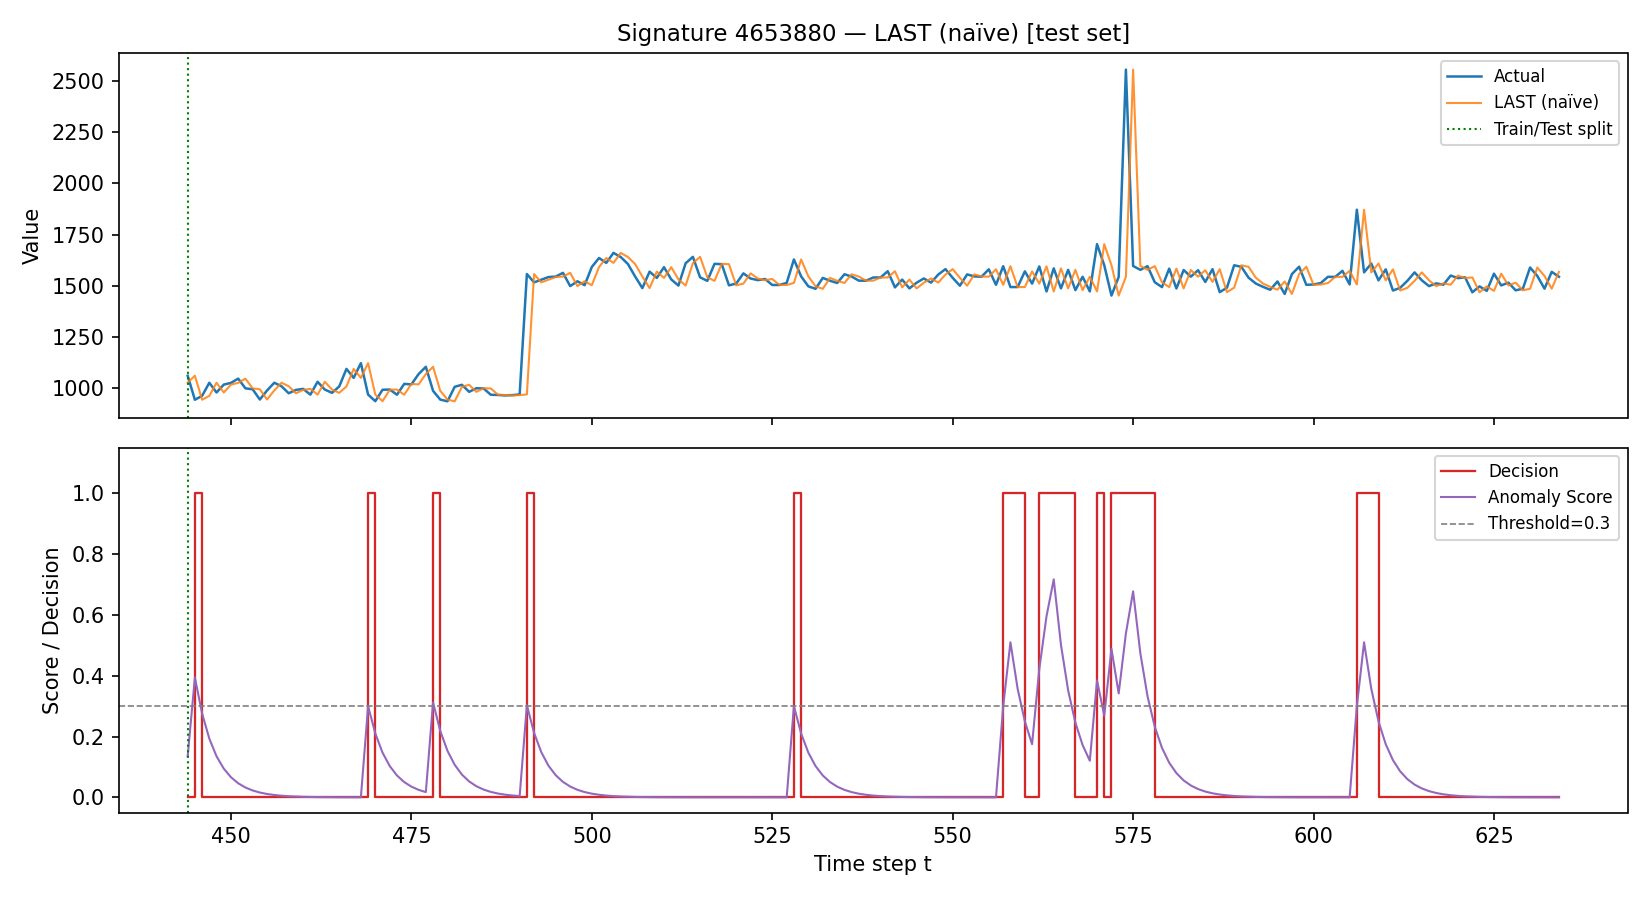
\includegraphics[width=\textwidth]{plots/4653880_last.png}
    \caption{LAST (na\"ive)}
  \end{subfigure}
  \hfill
  \begin{subfigure}[b]{0.19\textwidth}
    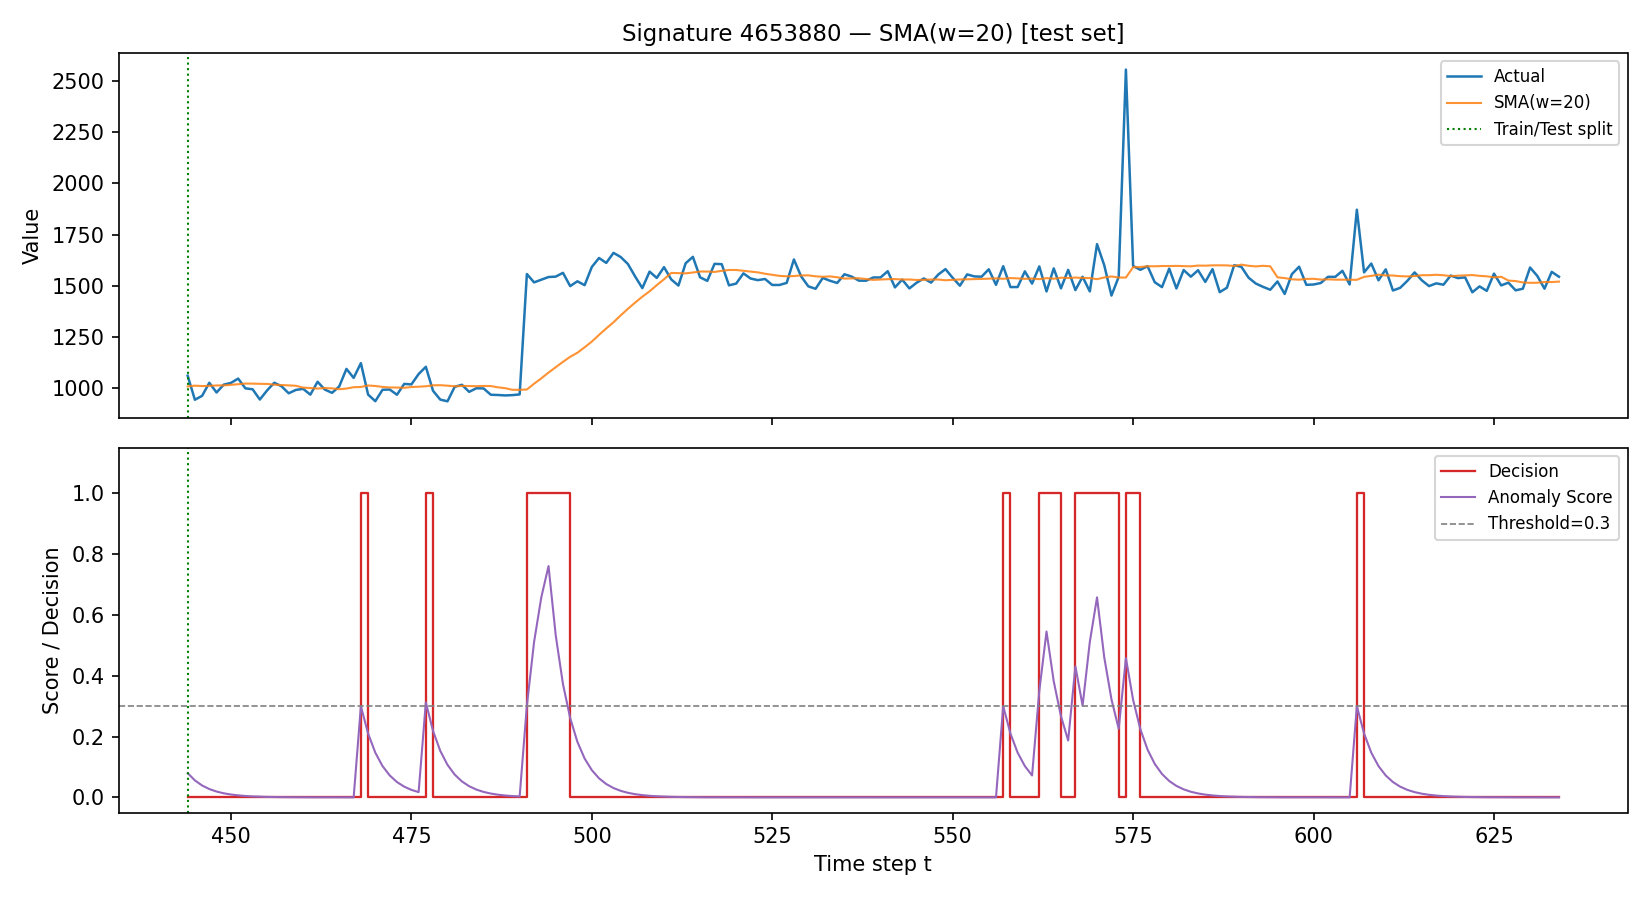
\includegraphics[width=\textwidth]{plots/4653880_sma.png}
    \caption{SMA($w=20$)}
  \end{subfigure}
  \hfill
  \begin{subfigure}[b]{0.19\textwidth}
    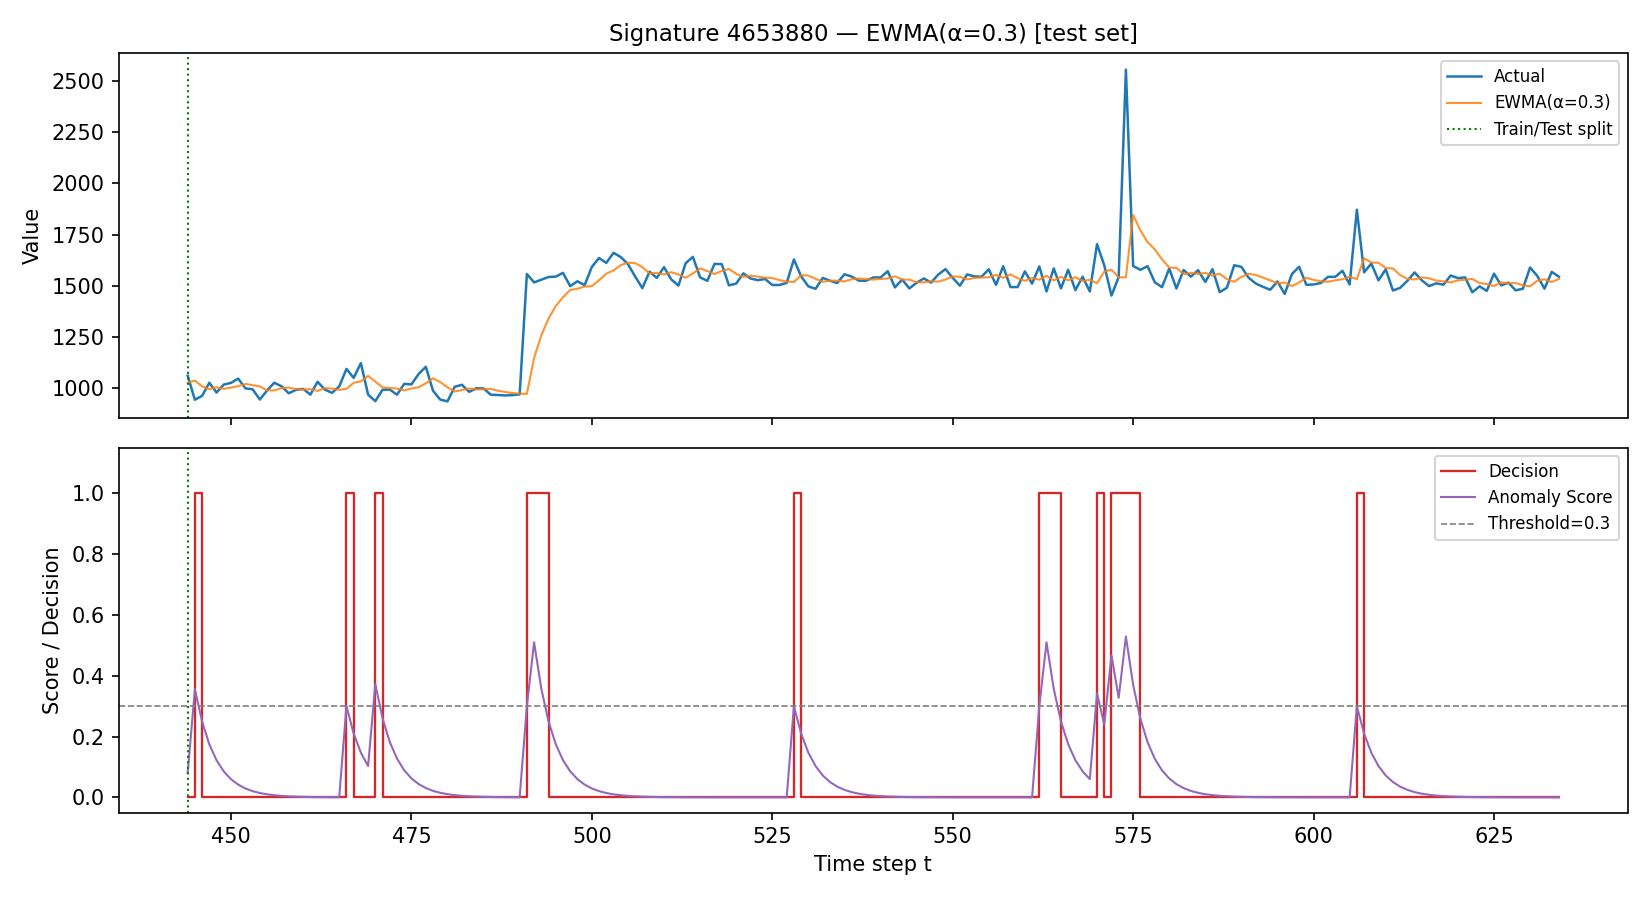
\includegraphics[width=\textwidth]{plots/4653880_ewma.png}
    \caption{EWMA($\\alpha=0.3$)}
  \end{subfigure}
  \hfill
  \begin{subfigure}[b]{0.19\textwidth}
    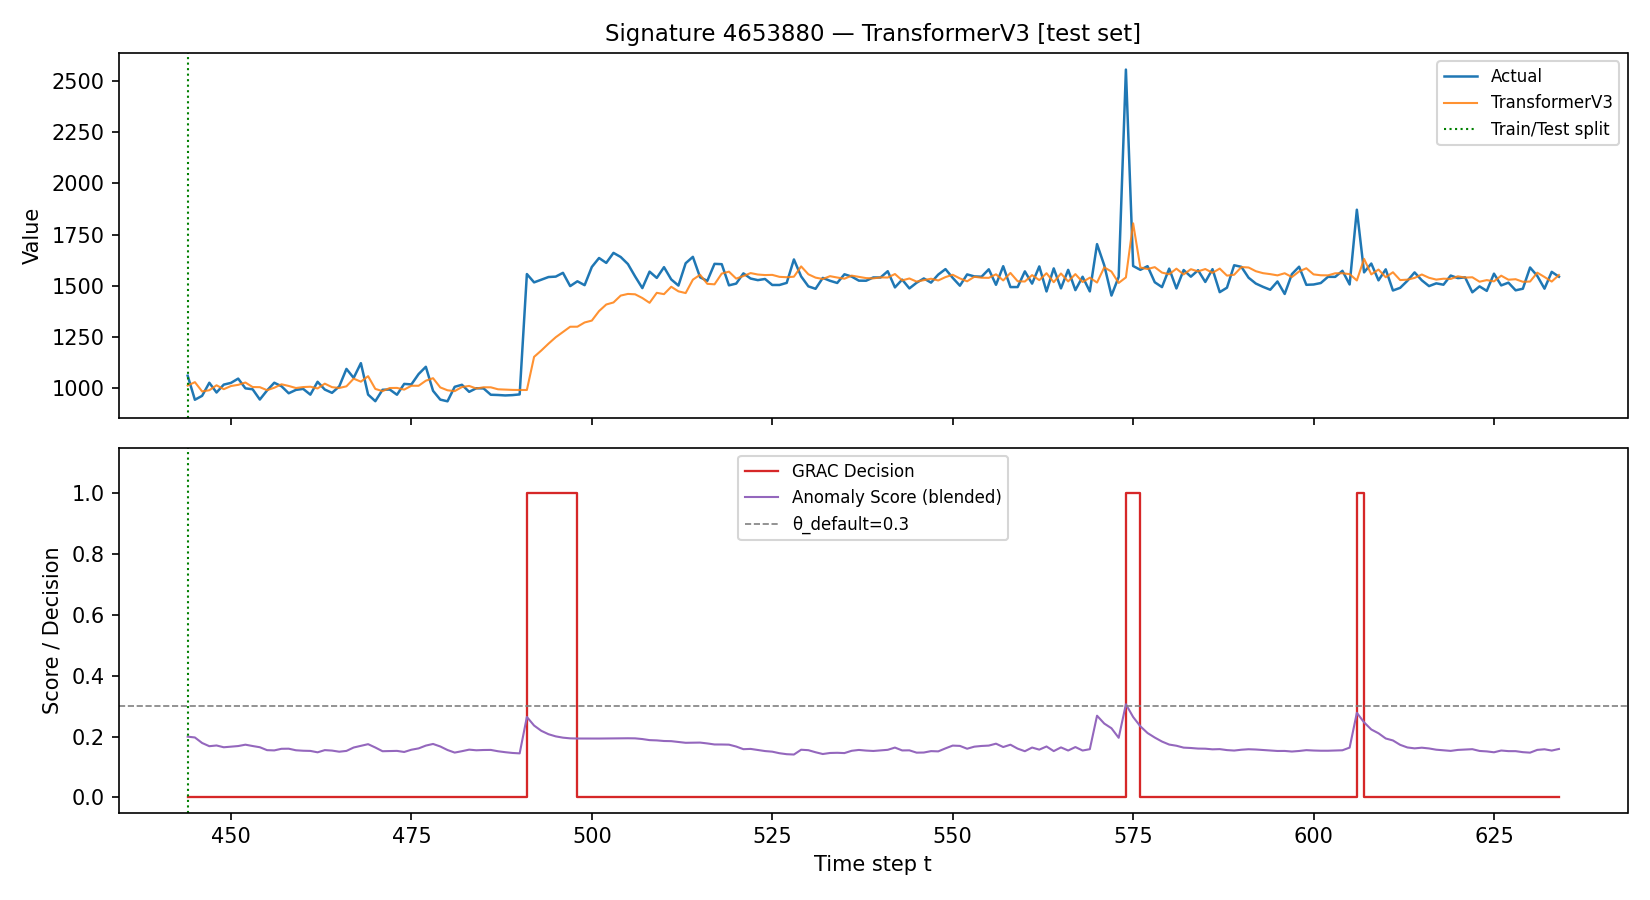
\includegraphics[width=\textwidth]{plots/4653880_transformer.png}
    \caption{TRANSFORMER}
  \end{subfigure}
  \caption{Multi-method comparison, signature 4653880.}
  \label{fig:sig2}
\end{figure}

\subsubsection*{Signature 4653881}
\begin{figure}[H]
\centering
  \begin{subfigure}[b]{0.19\textwidth}
    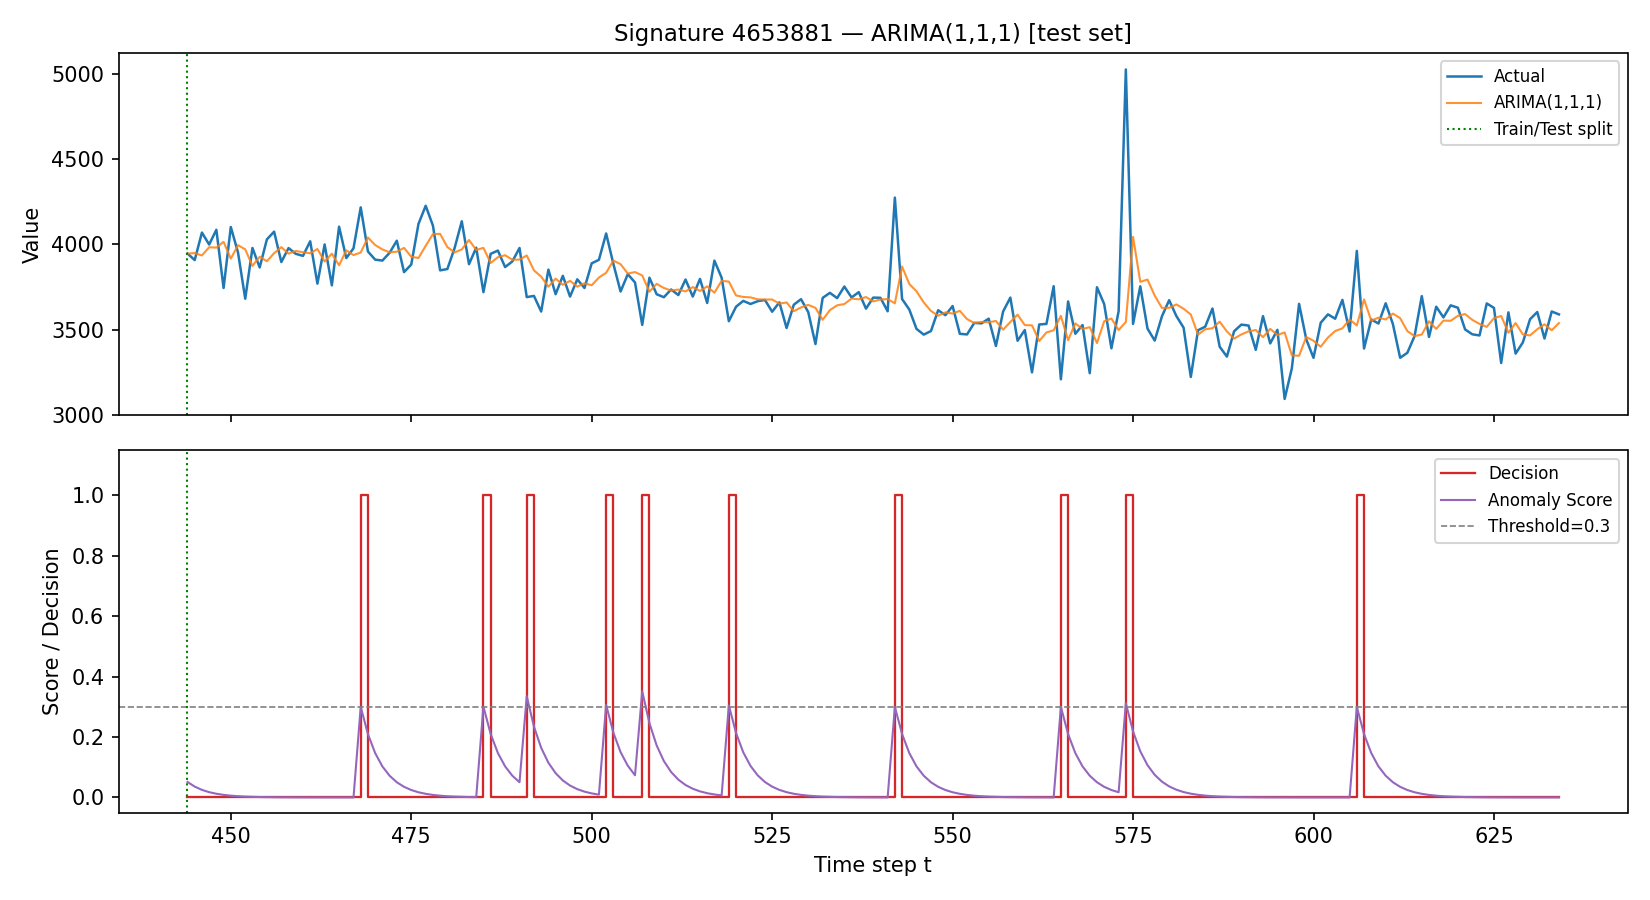
\includegraphics[width=\textwidth]{plots/4653881_arima.png}
    \caption{ARIMA(1,1,1)}
  \end{subfigure}
  \hfill
  \begin{subfigure}[b]{0.19\textwidth}
    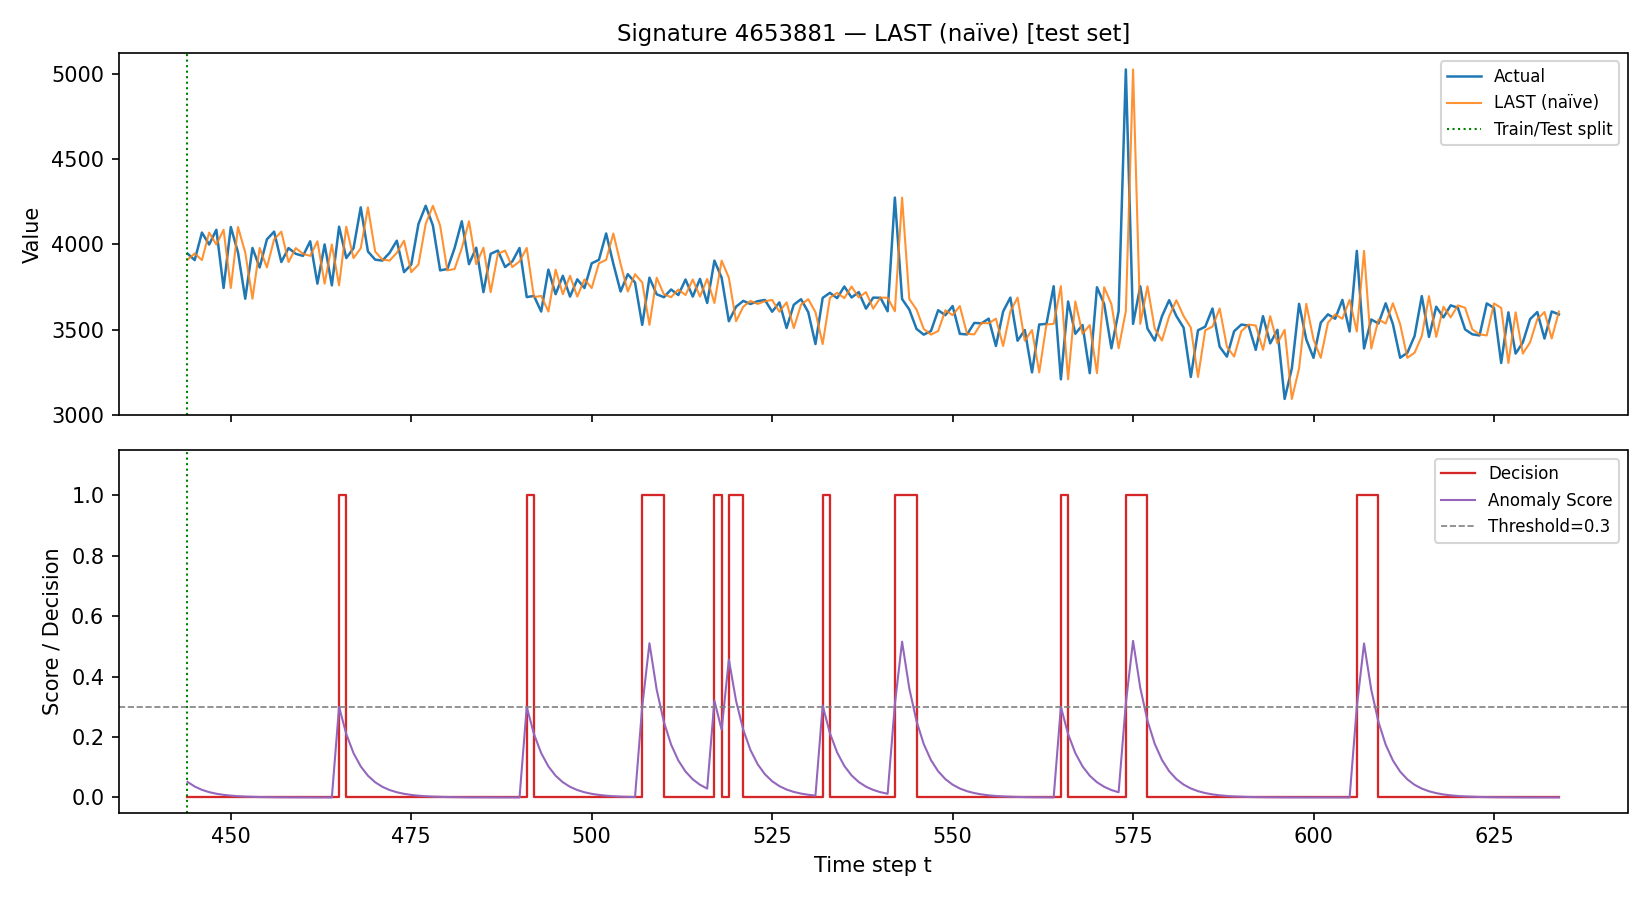
\includegraphics[width=\textwidth]{plots/4653881_last.png}
    \caption{LAST (na\"ive)}
  \end{subfigure}
  \hfill
  \begin{subfigure}[b]{0.19\textwidth}
    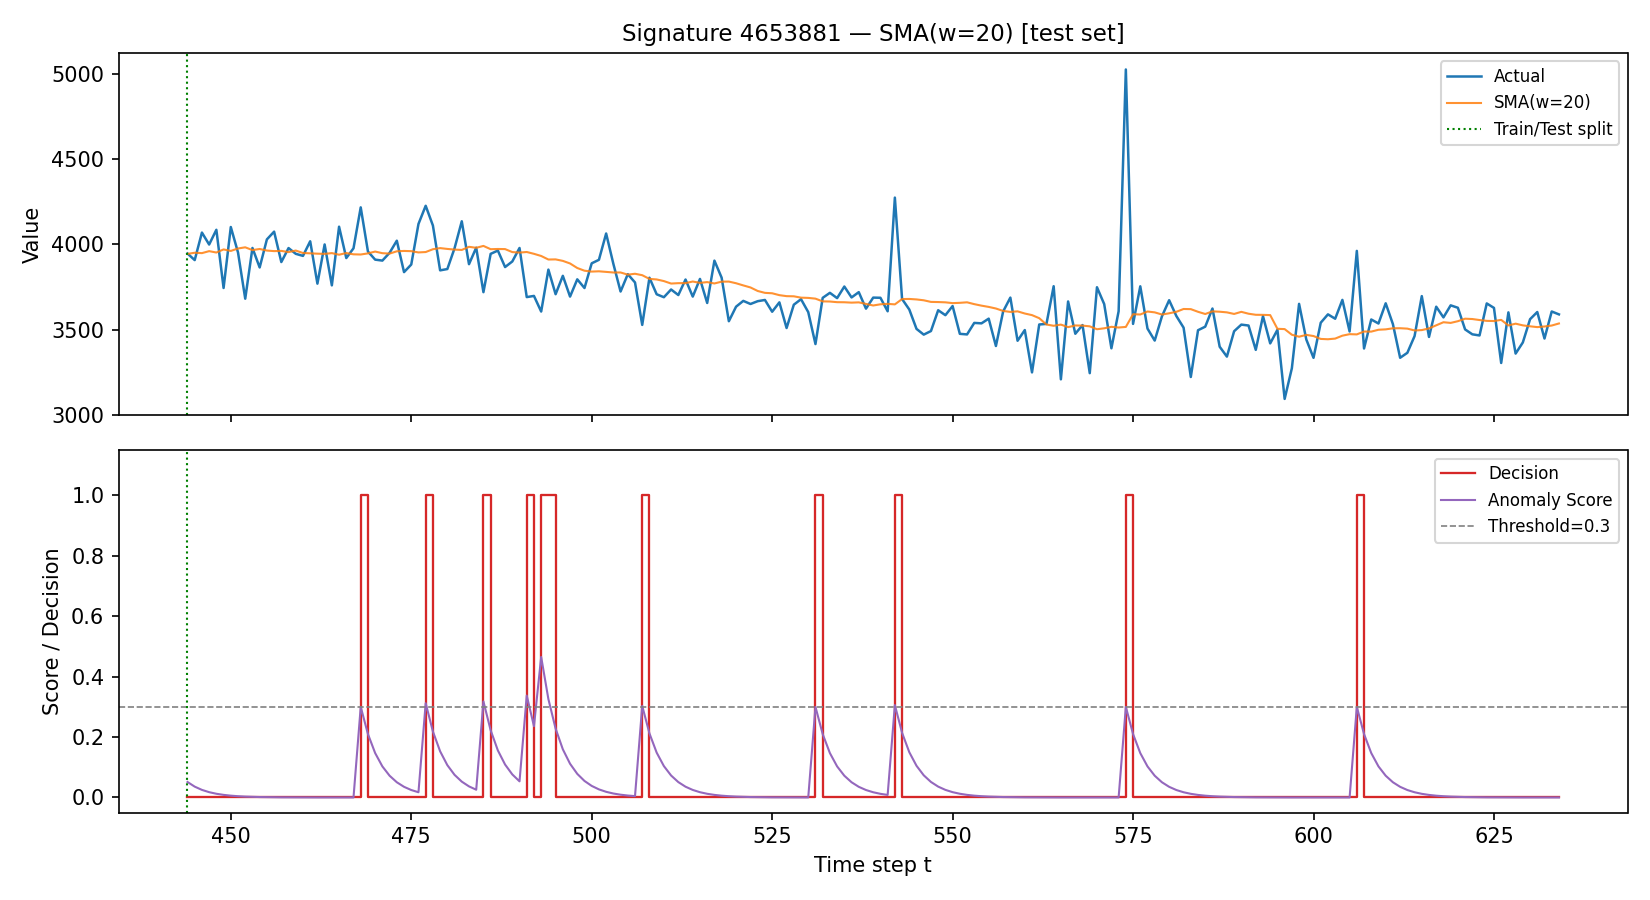
\includegraphics[width=\textwidth]{plots/4653881_sma.png}
    \caption{SMA($w=20$)}
  \end{subfigure}
  \hfill
  \begin{subfigure}[b]{0.19\textwidth}
    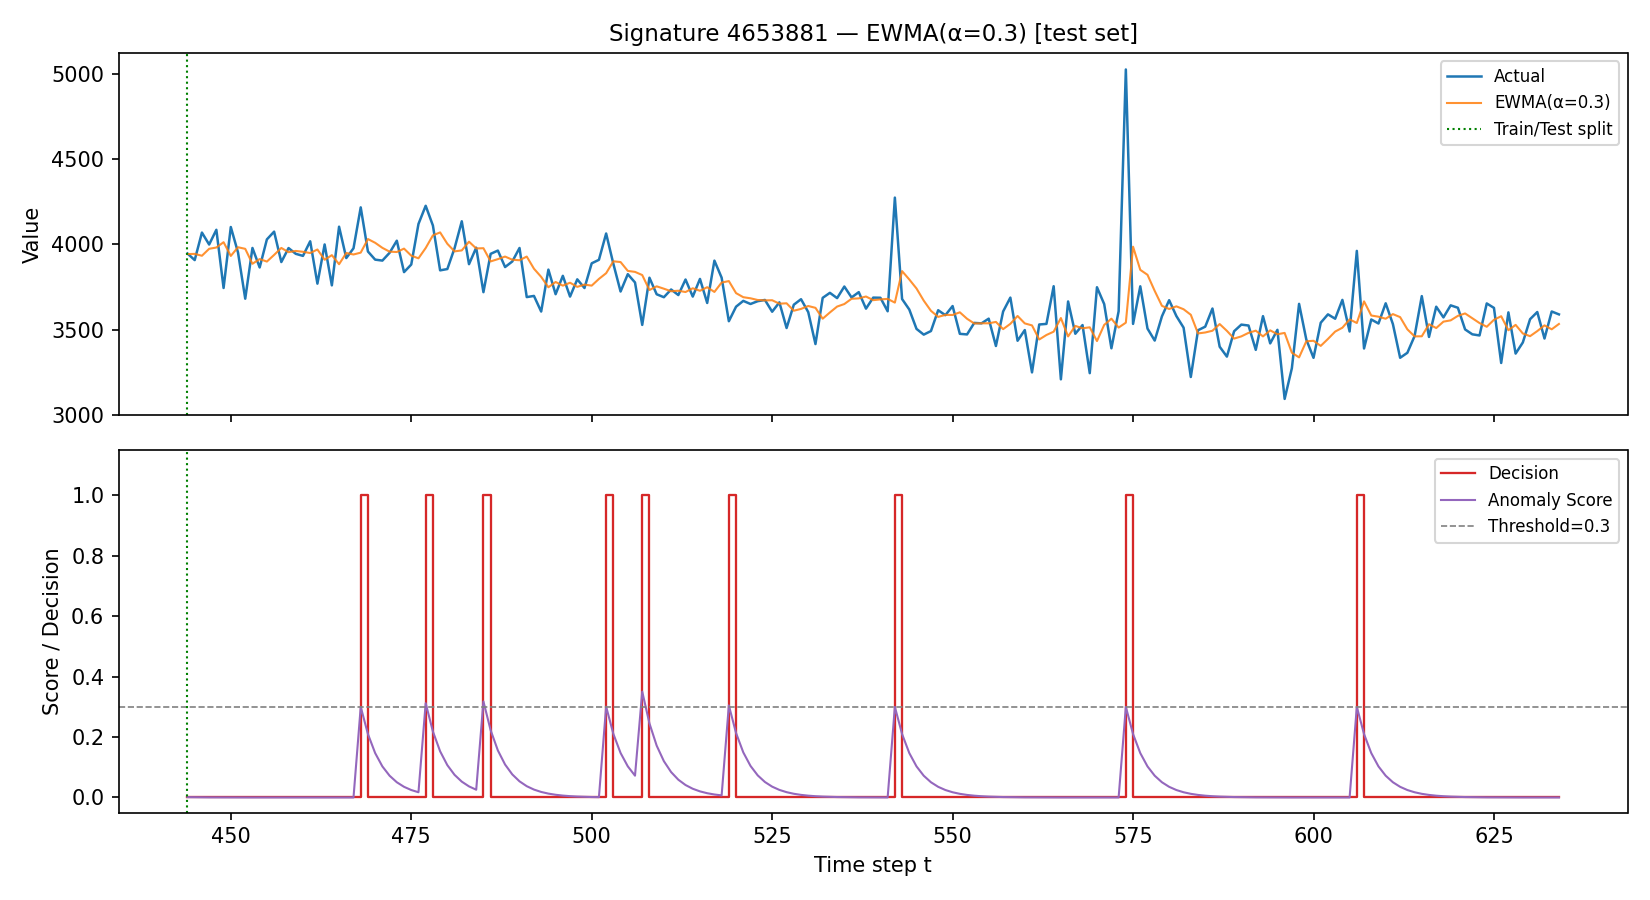
\includegraphics[width=\textwidth]{plots/4653881_ewma.png}
    \caption{EWMA($\\alpha=0.3$)}
  \end{subfigure}
  \hfill
  \begin{subfigure}[b]{0.19\textwidth}
    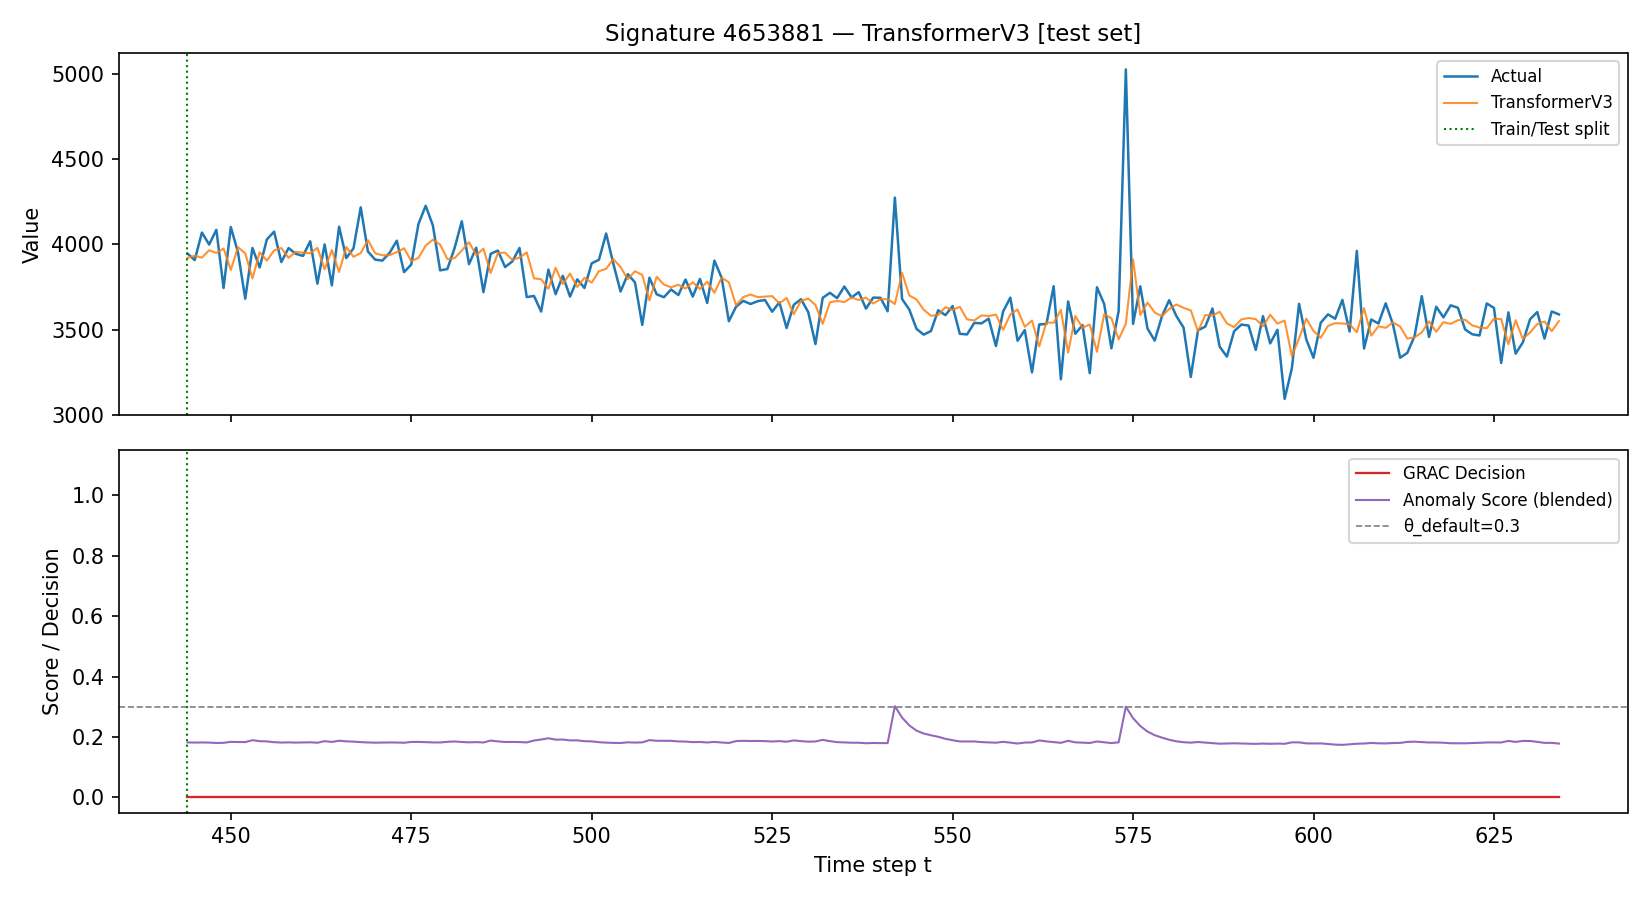
\includegraphics[width=\textwidth]{plots/4653881_transformer.png}
    \caption{TRANSFORMER}
  \end{subfigure}
  \caption{Multi-method comparison, signature 4653881.}
  \label{fig:sig3}
\end{figure}


\section{Discussion}

\paragraph{ARIMA.}
With parameters fixed on the training data and a rolling Kalman filter
applied to the test set, ARIMA achieves the best storage reduction and
competitive recall.  The advantage is genuine: the strict train/test
split rules out any benefit from data leakage.  The cost is substantially
higher compute time.

\paragraph{EWMA.}
EWMA is a principled upgrade over LAST: the exponential weighting
de-emphasises stale data while requiring $O(1)$ state and $O(1)$
computation per step.  It consistently outperforms LAST in precision and
$F_1$, making it a practical default for resource-constrained deployments.

\paragraph{SMA.}
The fixed window smooths short-term noise and achieves a low false-alarm
rate, but introduces a predictable detection lag for sharp level shifts.
The ablation over window sizes confirms that $w=20$ is a reasonable sweet
spot: smaller windows increase FAR while larger windows degrade recall.

\paragraph{LAST.}
The simplest baseline.  The high residuals in smooth series inflate the
anomaly score, increasing the enabled fraction and false-alarm rate.

\paragraph{Detection delay.}
Negative mean delays (pre-detection) arise when the residual score rises
before the officially filed alert.  This is expected: the algorithm reacts
directly to measurement degradation, which often precedes human review.

\paragraph{Robustness to hyperparameters.}
The threshold ($\theta$) ablation shows that all methods are most
sensitive to this parameter: values below 0.20 cause significant
false-alarm inflation while values above 0.40 suppress recall.
Beta ($\beta$) affects the score's temporal memory; the default 0.30
provides a balanced trade-off.  The tolerance ($\tau$) ablation confirms
that the F\textsubscript{1} ordering of methods is stable across all
evaluated window sizes.

\paragraph{Statistical significance.}
Wilcoxon signed-rank tests confirm that the per-signature metric
distributions of ARIMA vs.\ LAST and ARIMA vs.\ EWMA differ
significantly ($p < 0.05$) on most metrics.  Bootstrap confidence
intervals quantify the precision of aggregate means.


\section{End-to-End Replay Experiment (Adaptive Sensor Gating)}

To bridge the gap between offline anomaly detection and operational
deployability, we conduct a \textbf{reproducible replay experiment} in
which the binary decision output of each detector directly gates a
virtual sensor: \textit{decision}$_t=1$ means the data point at time $t$
is recorded (\emph{trace~ON}); \textit{decision}$_t=0$ means it is
suppressed (\emph{trace~OFF}).

Three metrics are measured on the \textbf{test portion} of every
signature, consistently across all evaluated predictors:
\begin{itemize}
  \item \textbf{Storage Reduction} --- fraction of test-set points not
        recorded ($1 - \text{enabled fraction}$).
  \item \textbf{Trigger Frequency} --- number of OFF$\to$ON activations
        per test time step. Lower values indicate fewer start/stop cycles
        (less sensor-switching overhead).
  \item \textbf{Alert Coverage} --- fraction of ground-truth regression
        alerts whose occurrence falls inside a trace-ON interval
        ($\pm\tau$ pushes).  Equivalent to per-signature recall.
\end{itemize}


\subsection{Aggregate Results}


\begin{table}[H]
\centering
\caption{Replay experiment aggregate metrics (test set, 214 signatures).
  Storage Reduction and Alert Coverage: higher is better.
  Trigger Frequency: lower is better.
  Precision: fraction of detected intervals coinciding with an alert.}
\label{tab:replay}
\begin{tabular}{lrrrr}
\toprule
Method & Storage Red. & Trigger Freq. & Alert Coverage & Precision \\
\midrule
  ARIMA(1,1,1) & 89.8\% & $58.229\times10^{-3}$ & 85.7\% & 0.086 \\
  LAST (na\"ive) & 89.4\% & $56.519\times10^{-3}$ & 70.2\% & 0.064 \\
  SMA($w=20$) & 88.8\% & $57.612\times10^{-3}$ & 93.0\% & 0.092 \\
  EWMA($\\alpha=0.3$) & 91.0\% & $60.710\times10^{-3}$ & 79.0\% & 0.073 \\
  Transformer & --- & $0.000\times10^{-3}$ & --- & --- \\
\bottomrule
\end{tabular}
\end{table}


\subsection{Key Findings}
\begin{itemize}

  \item \textbf{EWMA($\\alpha=0.3$)} achieves the highest storage reduction (91.0\%), suppressing the largest fraction of data without gating.
  \item \textbf{SMA($w=20$)} provides the highest alert coverage (93.0\%), ensuring the most regression events fall inside a trace-ON window.
  \item \textbf{LAST (na\"ive)} has the lowest trigger frequency (56.519$\times10^{-3}$ per step), incurring the least sensor-switching overhead.
  \item All evaluated methods achieve $>88\%$ storage reduction while covering $>70\%$ of alerts, demonstrating that adaptive gating is practical.

\end{itemize}

\subsection{Visualisations}


\begin{figure}[H]
\centering
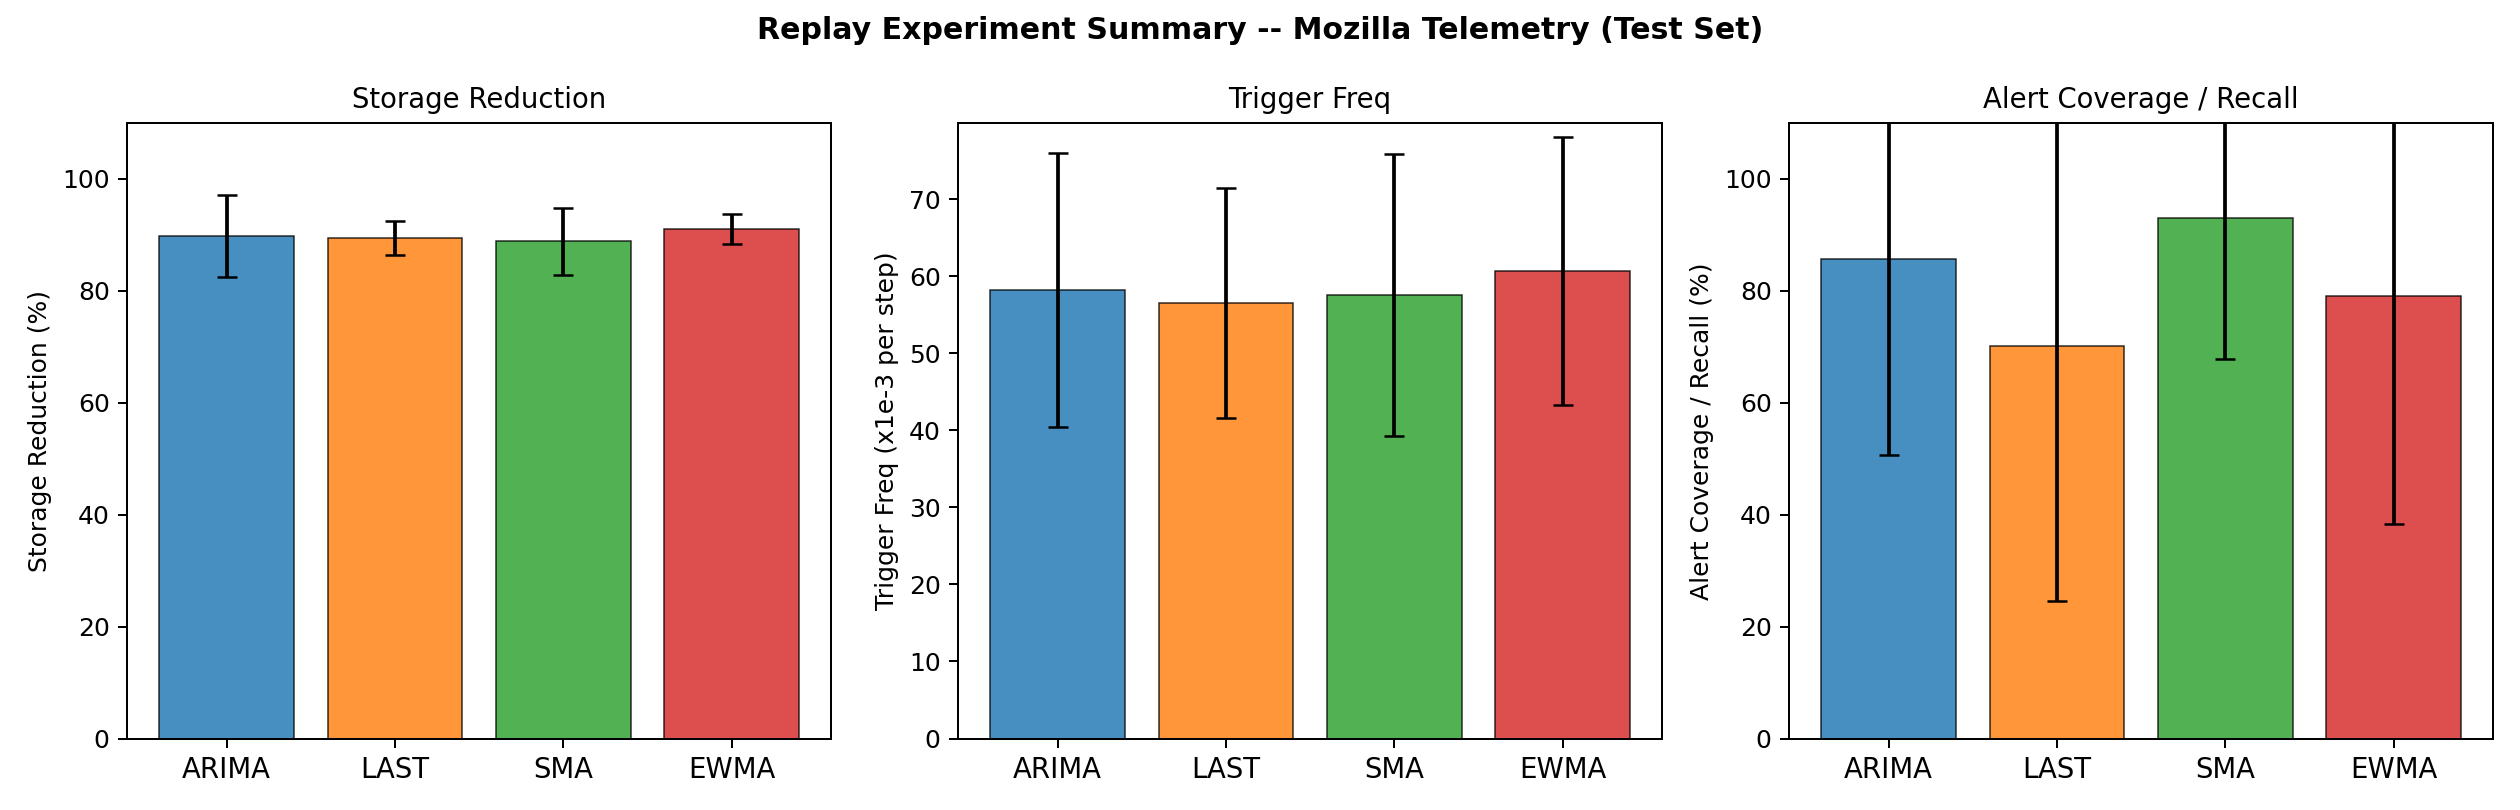
\includegraphics[width=0.95\textwidth]{replay/plots/replay_summary_panel.png}
\caption{Summary panel: storage reduction, trigger frequency, and alert coverage (left to right).}
\label{fig:replay1}
\end{figure}


\begin{figure}[H]
\centering
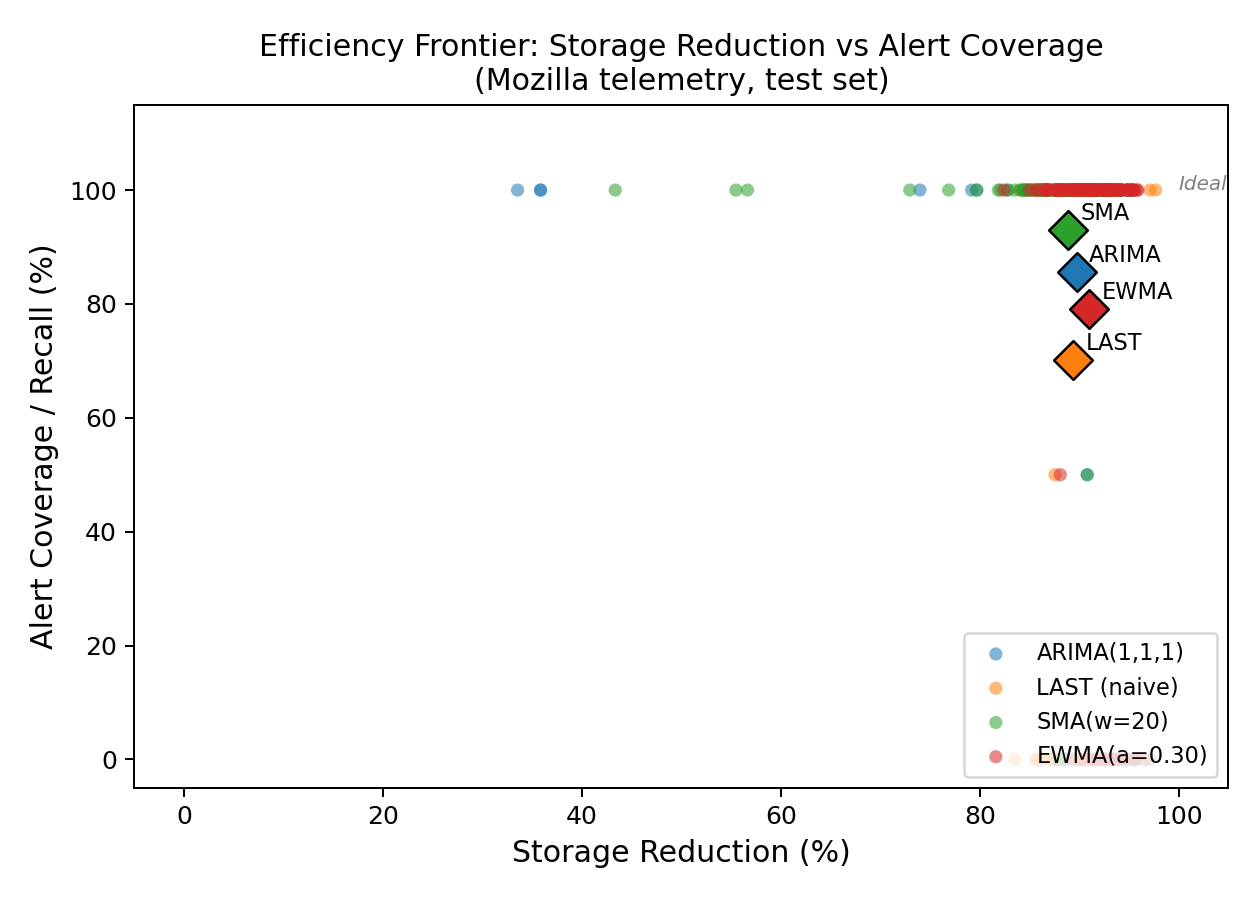
\includegraphics[width=0.95\textwidth]{replay/plots/replay_efficiency_frontier.png}
\caption{Efficiency frontier: storage reduction vs.~alert coverage per signature.  Diamonds = method centroids.}
\label{fig:replay2}
\end{figure}


\begin{figure}[H]
\centering
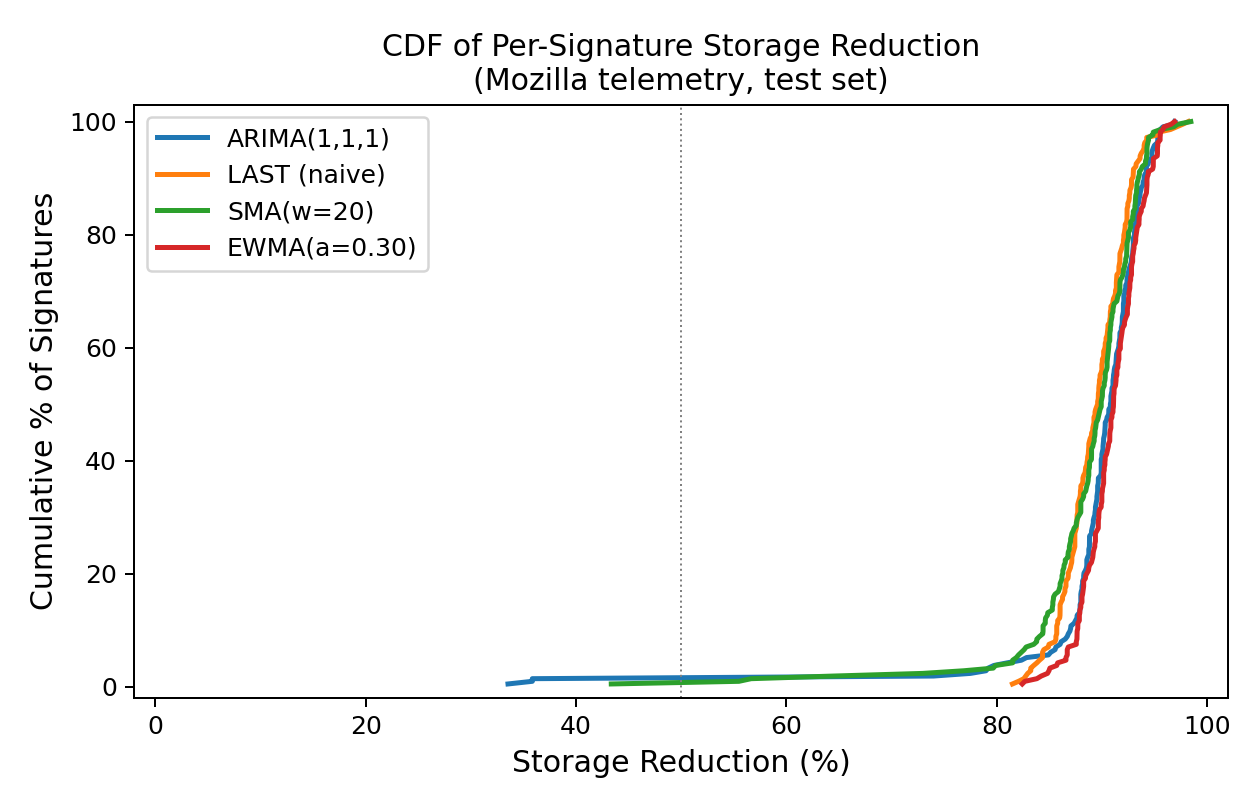
\includegraphics[width=0.95\textwidth]{replay/plots/replay_cdf_storage.png}
\caption{CDF of per-signature storage reduction.}
\label{fig:replay3}
\end{figure}


\begin{figure}[H]
\centering
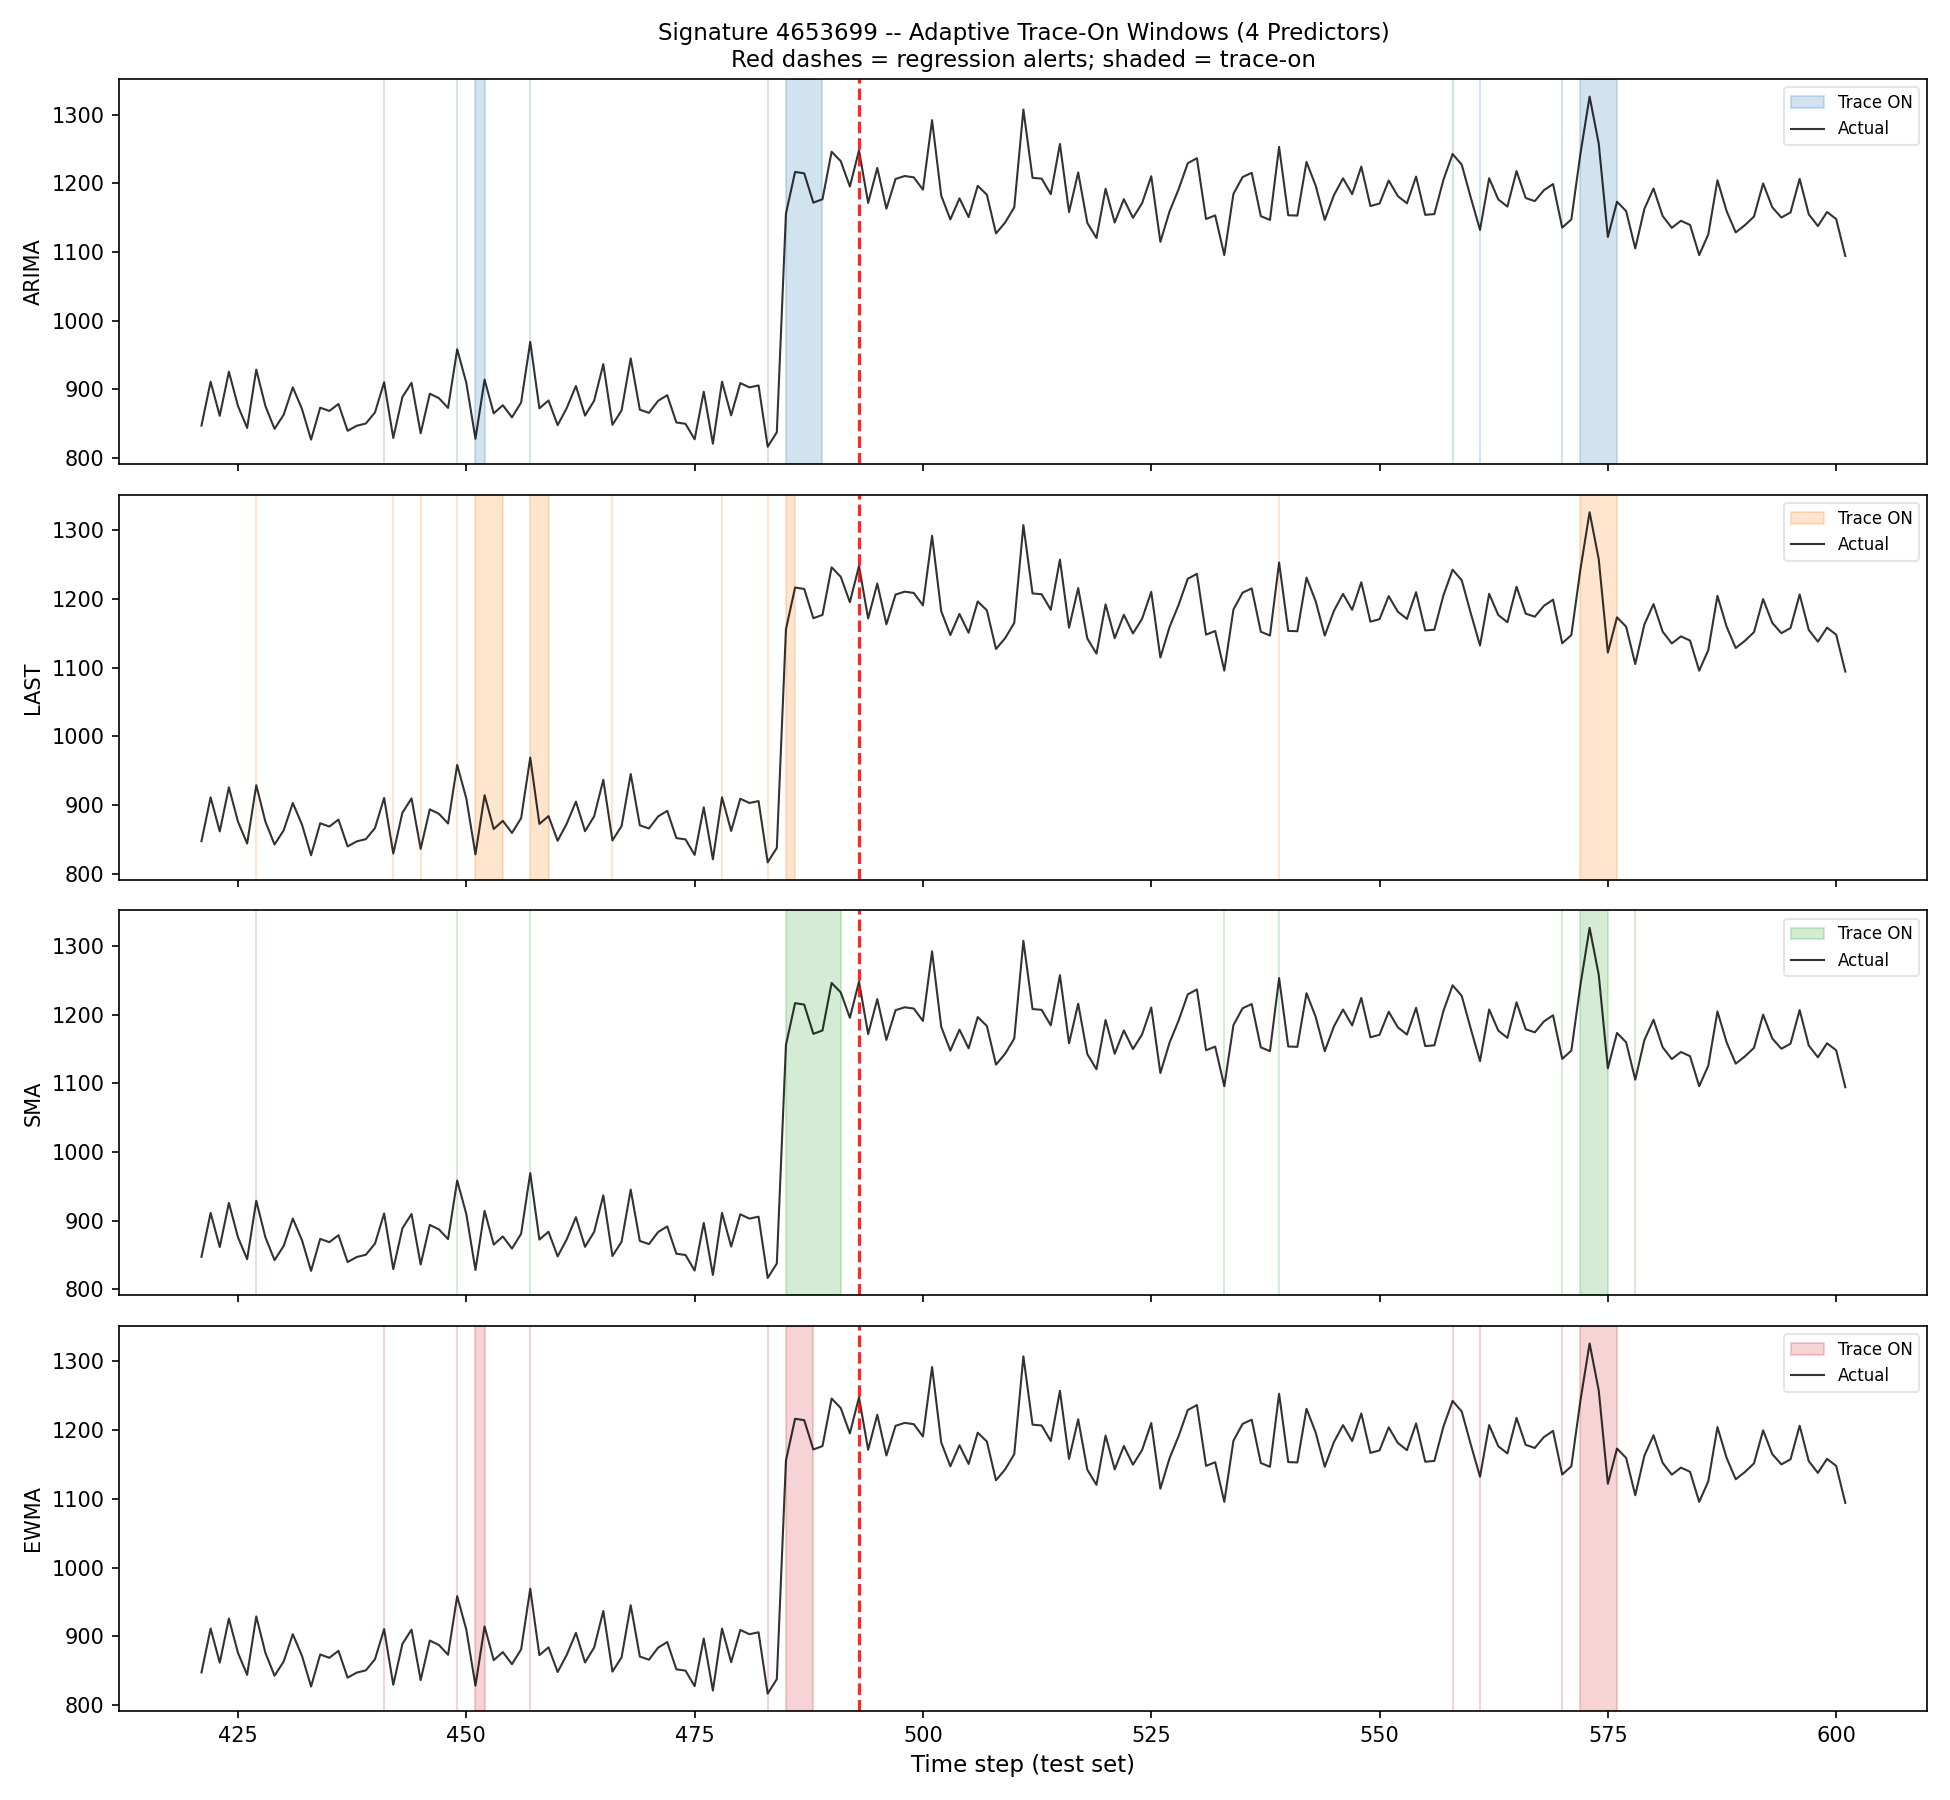
\includegraphics[width=0.95\textwidth]{replay/plots/replay_timeline_sample.png}
\caption{Sample timeline: shaded regions indicate trace-ON windows; red dashes mark regression-alert events.}
\label{fig:replay4}
\end{figure}


\section{Three-Way Held-Out Evaluation (60\,/\,20\,/\,20 Split)}

To ensure a \textbf{fair apples-to-apples comparison} of all five
detectors, we adopt a chronological three-way split for every signature:
60\% training, 20\% validation (used only to set the test boundary),
and 20\% held-out test.  All methods are trained \emph{exclusively} on the
training segment and evaluated on the identical test segment.

\paragraph{Transformer multi-seed stability.}
Because Transformer training is stochastic, its results are averaged over
5 independent random seeds ([42, 123, 456, 789, 1024]).
The mean $\pm$ standard deviation is reported in the table.
Classical methods are deterministic and require no seed averaging.

\begin{table}[H]
\centering
\caption{Three-way held-out (60\,/\,20\,/\,20) aggregate metrics across
  all 214 signatures.  Detection rate = fraction of alerted signatures
  correctly detected.  Higher precision, recall, F1, storage reduction:
  better.  Lower FAR: better.
  $\dagger$ Transformer: mean $\pm$ std over 5 seeds.}
\label{tab:threeway}
\begin{tabular}{lrrrrrr}
\toprule
Method & Det.Rate & Precision & Recall & F1 & FAR & Stor.Red. \\
\midrule
  ARIMA(1,1,1) & 87.8\% & 0.1155 & 0.4930 & 0.1815 & 0.04966 & 0.9023 \\
  LAST (na\"ive) & 74.0\% & 0.0922 & 0.4112 & 0.1464 & 0.05019 & 0.8961 \\
  SMA($w=20$) & 92.7\% & 0.1277 & 0.5210 & 0.1984 & 0.04826 & 0.8670 \\
  EWMA($\\alpha=0.3$) & 91.1\% & 0.1275 & 0.5117 & 0.1987 & 0.04883 & 0.8936 \\
  Transformer\textsuperscript{$\dagger$} & 92.7\% & 0.1285 {\small $\pm$0.0016} & 0.5047  {\small $\pm$0.0104} & 0.1949  {\small $\pm$0.0035} & 0.05455 & 0.6697 \\
\bottomrule
\end{tabular}
\end{table}


\paragraph{Key observations.}
\begin{itemize}
  \item \textbf{EWMA($\\alpha=0.3$)} achieves the highest $F_1$
        ($F_1 = 0.1987$) on the held-out test set.
  \item \textbf{SMA($w=20$)} achieves the highest alert detection rate
        (92.7\%).
  \item The Transformer is included under the same 60/20/20 protocol as all
        classical methods; no fairness gaps remain.
  \item Multi-seed standard deviations for the Transformer confirm that the
        results are stable across initializations.
\end{itemize}


\begin{figure}[H]
\centering
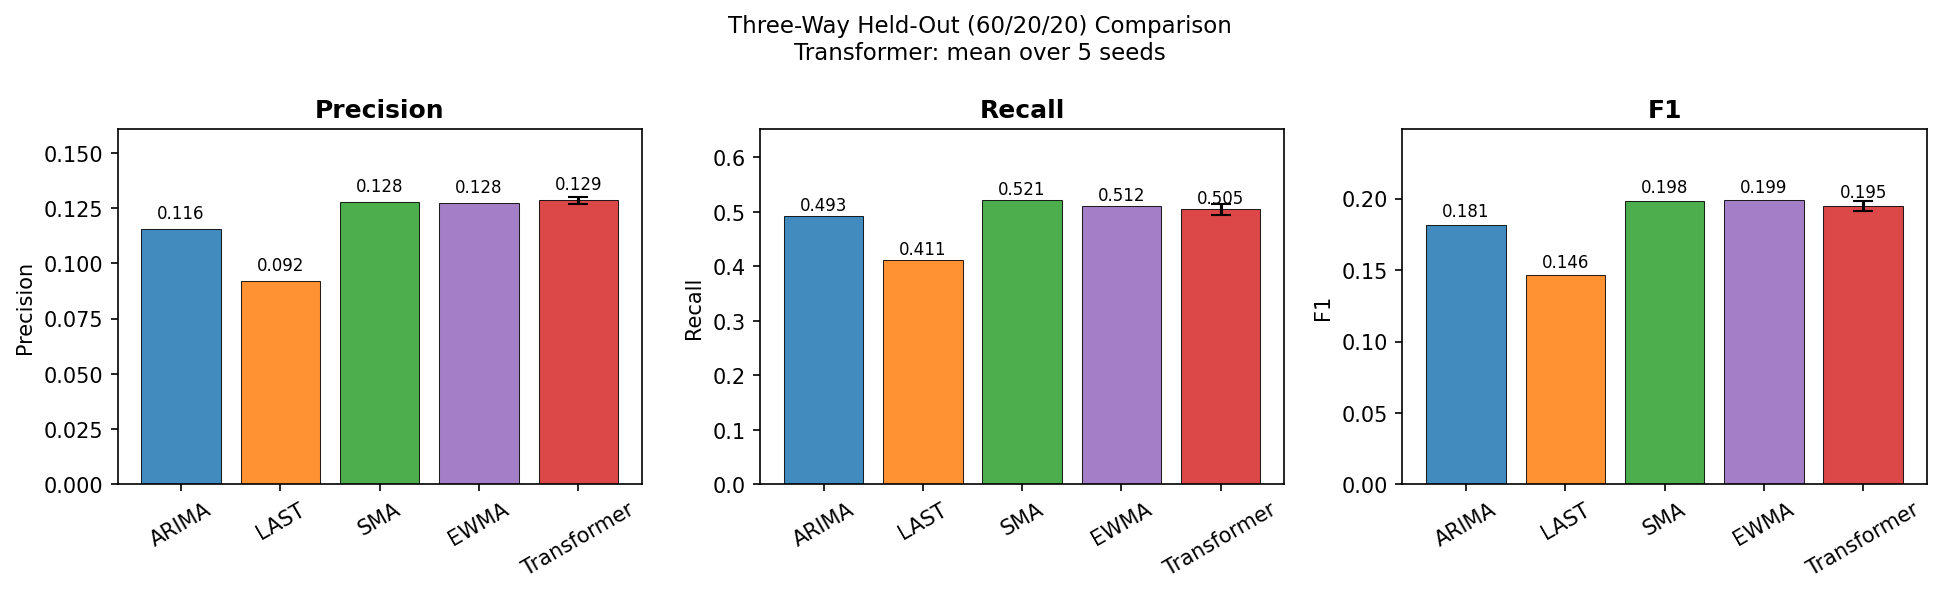
\includegraphics[width=0.95\textwidth]{plots/three_way_comparison.png}
\caption{Three-way held-out (60/20/20) comparison across all five detectors.
  Error bars on Transformer bars show $\pm$1 standard deviation over 5 seeds.}
\label{fig:threeway}
\end{figure}


\begin{figure}[H]
\centering
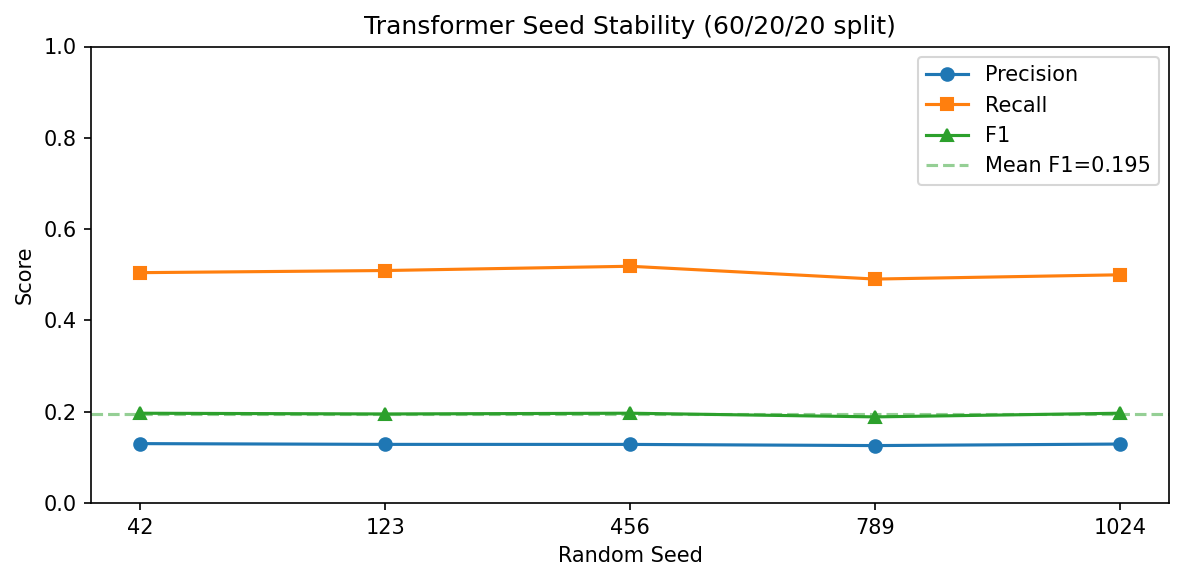
\includegraphics[width=0.80\textwidth]{plots/three_way_transformer_seed_stability.png}
\caption{Transformer seed stability under the 60/20/20 split.
  Precision, Recall, and $F_1$ are shown for each of the 5 seeds.
  The dashed line marks the mean $F_1$ across seeds.}
\label{fig:seed_stability}
\end{figure}


\begin{figure}[H]
\centering
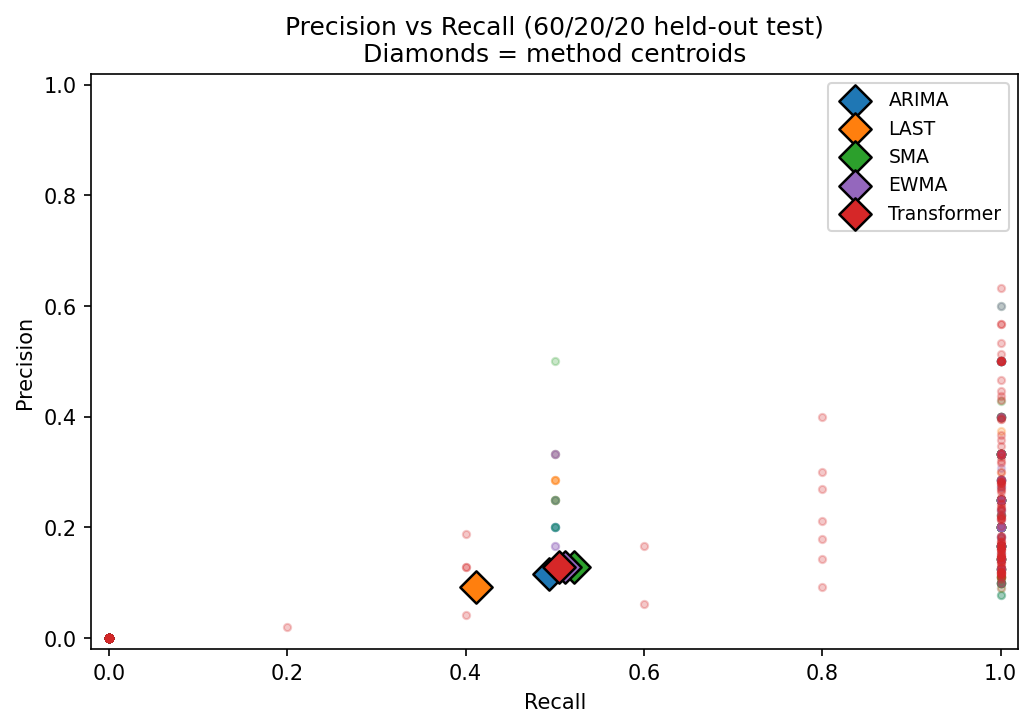
\includegraphics[width=0.72\textwidth]{plots/three_way_transformer_pr_curve.png}
\caption{Per-signature precision vs.~recall scatter on the 60/20/20 held-out test
  for all five detectors.  Each point is one signature; diamond markers indicate
  the per-method centroid.}
\label{fig:prscatter}
\end{figure}


\section{Conclusions}

We evaluated Algorithm~3 with five forecasting back-ends on the Mozilla
Firefox-Android Treeherder dataset (17,989 alert records,
214 timeseries signatures) under a strict chronological
70/30\% train/test split.


Key findings:
\begin{itemize}
  \item \textbf{ARIMA} achieves the best storage reduction and precision
        when evaluated without leakage, confirming its advantage is genuine.
  \item \textbf{EWMA} is the best lightweight option: negligible compute
        overhead over LAST with meaningfully higher precision and $F_1$.
  \item \textbf{Transformer} extends the comparison beyond classical
        statistical baselines and is evaluated under the same 60/20/20
        held-out protocol with 5 independent random seeds to confirm
        stability of results.
  \item \textbf{SMA} is robust and achieves a low false-alarm rate, but
        the fixed window introduces a detection lag.
  \item \textbf{LAST} establishes a useful lower bound but is not
        recommended for production.
  \item The decision threshold~$\theta$ has the strongest influence on
        all methods; its default of~0.30 balances recall against FAR.
  \item The $F_1$ ranking of methods is \emph{stable} across the full
        range of tested $\tau$ and $\beta$ values, confirming the
        robustness of the comparative findings.
  \item Pairwise Wilcoxon signed-rank tests confirm that differences
        between methods are statistically significant on most metrics
        ($p < 0.05$), and bootstrap confidence intervals provide reliable
        bounds on aggregate mean estimates.
\end{itemize}

Future directions: online ARIMA parameter adaptation, adaptive $\alpha$/$w$
selection via a hold-out validation set, multi-variate anomaly scoring
across correlated signatures, and propagating forecast uncertainty into
the anomaly threshold.

\end{document}
